\documentclass[trackchanges]{aastex62}
\usepackage{amsmath}
\usepackage{mathtools}
\usepackage{color}
\usepackage{hyperref}
\usepackage[normalem]{ulem}

\newcommand\latex{La\TeX}
\newcommand{\dd}{{\mathrm d}}
\newcommand{\rmsub}[1]{_\mathrm{#1}}
\newcommand{\bmu}{\boldsymbol{\mu}}
\newcommand{\beps}{\boldsymbol{\varepsilon}}
\newcommand{\blam}{\boldsymbol{\Lambda}}
\newcommand{\vx}[1]{{\bf {#1}}}
\newcommand{\vxhat}[1]{{\bf {\hat{#1}}}}
\newcommand{\pkgname}{\texttt{amlc}}

\graphicspath{{./}{figures/}}

\shortauthors{Tchernyshyov}

\begin{document}

\title{Analytic marginalization of absorption line continua}

\author[0000-0003-0789-9939]{Kirill Tchernyshyov}
\affiliation{Department of Physics and Astronomy, Johns Hopkins University, 3400 N. Charles Street, Baltimore, MD 21218, USA}
\correspondingauthor{Kirill Tchernyshyov}
\email{ktcherny@gmail.com}

\begin{abstract}
Absorption line spectroscopy is a powerful way of measuring properties of stars and the interstellar medium.
Absorption spectra are often analyzed manually, an approach that limits reproducibility and which cannot practically be applied to modern datasets consisting of thousands or even millions of spectra.
Simultaneous probabilistic modeling of absorption features and continuum shape is a promising approach for automating this analysis.
Existing implementations of this approach use numerical methods such as Markov chain Monte Carlo (MCMC) to marginalize over the continuum parameters.
Numerical marginalization over large numbers of continuum parameters is too slow to be convenient for exploratory analysis, can increase the dimensionality of an inference problem beyond the capacity of simple MCMC samplers, and is in general impractical for the analysis of large datasets.
When continua are parameterized as linear functions such as polynomials or splines, it is possible to reduce continuum parameter marginalization to an integral over a multivariate normal distribution, which has a known closed form.
In addition to speeding up probabilistic modeling, analytic marginalization makes it trivial to marginalize over continuum parameterizations and to combine continuum description marginalization with optimization for absorption line parameters.
These new possibilities allow automatic, probabilistically justified continuum placement in analyses of large spectroscopic datasets.
We compare the accuracy to within which absorption line parameters can be recovered using different continuum placement methods and find that marginalization is in many cases an improvement over other methods.
We implement analytic marginalization over linear continuum parameters in the open-source package \pkgname.
\end{abstract}

\keywords{methods: statistical, techniques: spectroscopic}

\section{Introduction}
\label{sec:introduction}
Absorption lines contain information on the composition and properties of interstellar matter (ISM) and stellar atmospheres.
To extract this information, it is necessary to decompose the spectrum into absorption features and the intrinsic flux, typically referred to as the continuum, produced by the illuminating background source towards which the absorption is seen.
The most common way of doing this separation has been manually finding regions in a spectrum that do not contain absorption features, fitting a function to these regions, and using this function to interpolate over the absorption features.
Given the longevity and popularity of this approach, it is clear that it can produce acceptable results.
It does, however, have two important weaknesses.
The first is that every spectrum must be examined and interacted with by a human.
This cannot efficiently be done for datasets containing thousands or even millions of spectra.
The second is that it is unlikely that the absorption parameter estimator this procedure implicitly defines uses data efficiently.
There is variance between analyses done by different humans as well as between analyses done by the same human at different times.
If there is a subset of analysts whose estimates are the most accurate and precise, then the estimates of the rest are using the available data inefficiently.

An alternative approach is to infer absorption line and continuum parameters simultaneously.
To improve the accuracy of the inferred absorption line parameters, it can be useful to marginalize over, rather than fit for, the continuum parameters.
This has been done in packages meant for the analysis of absorption lines from both the ISM (\texttt{BayesVP}, \citealt{Liang:2018kq}) and stellar atmospheres (\texttt{Starfish}, \citealt{2015ApJ...812..128C}, and \texttt{sick}, \citealt{2016ApJS..223....8C}).
In these packages, continuum parameter marginalization is done numerically, using Markov chain Monte Carlo (MCMC).
As the authors of two of these packages point out, including large numbers of continuum parameters in MCMC sampling leads to long convergence and autocorrelation times.
To keep the number of continuum parameters low, these packages either do not support (\texttt{BayesVP}) or advise against (\texttt{sick}) including continuum parameters when simultaneously analyzing multiple spectral segments.

Even when there are few continuum parameters, using MCMC to analyze a modern spectroscopic dataset consisting of thousands or even millions of spectra will be computationally demanding.
Probablistic analyses of comparable numbers of photometric observations \citep[e.g.][]{2015ApJ...810...25G,2016ApJ...826..104G} require months or years of computation time.
A single spectrum contains orders of magnitude more data points than a single set of photometric observations, which comes with an at least linearly proportional increase in required computation time.

In the packages discussed above and in much of the absorption line analysis literature, the continuum is assumed to be a low order polynomial or spline.
{\bf Polynomials and splines are non-linear functions of their $x$-variable, in this case wavelength, but linear functions of their coefficients.
For example, a quadratic function, $f(x) = a x^2 + b x + c$, is non-linear in $x$ but linear in $a$, $b$, and $c$.
The same is true of any function that can be expressed as a linear combination of fixed, possibly non-linear functions of $x$.}
This linearity means that if some additional assumptions hold, it is possible to marginalize over these coefficients analytically.

Analytic marginalization has several advantages over numerical marginalization.
First, it can speed up MCMC-based inference for absorption line parameters by reducing the dimensionality of the problem.
Second, the ability to evaluate the continuum parameter-marginalized likelihood function and its gradient makes it possible to do optimization, rather than sampling, for the absorption parameters while still keeping the robustness provided by marginalizing over continuum parameters.
Finally, it makes marginalization over different possible continuum parameterizations computationally trivial---simply sum together continuum-marginalized likelihoods that assume different parameterizations.
Marginalization over parameterizations allows an even greater degree of automation and systematization of absorption line inference.

{\bf The assumptions required for this particular form of analytic marginalization are: that the continuum can be expressed as a function that is linear in its parameters (not necessarily a polynomial or spline); that the priors on the parameters of this function are either improper uniform or (multivariate) normal; and that residuals from the model are normally distributed.}
If these assumptions hold, then, given a model for the absorption, the posterior probability distribution function of the continuum parameters is itself a multivariate normal distribution.
{\bf The first assumption, that the continuum can be expressed as a function that is linear in its parameters, is fulfilled by commonly used functions such as polynomials and splines.
One of the options given in the second assumption, that the priors on the parameters of this function are improper uniform, is made implicitly any time a continuum is fit without explicitly defining priors.
The third assumption, that residuals from the model are normally distributed, is made whenever a spectrum is analyzed as a set of continuous quantities, such as fluxes, rather than as a set of discrete photon counts.\footnote{Assuming that a spectrum consists of e.g. fluxes rather than photon counts does not require assuming that residuals are normally distributed, but normality has been assumed in every such instance known to the author.}}

The result of marginalizing over the continuum parameters is simply an update to the covariance matrix of the model residuals.
Conceptually, when a set of absorption line parameters is specified, the continuum parameters can be treated as additive, rather than multiplicative, linear nuisance parameters.
An explanation of marginalization over additive linear nuisance parameters in an astronomical context is given in \citet{2017RNAAS...1a...7L}.
This approach to marginalizing over multiplicative linear nuisance parameters has already been used for several astronomical applications, for example for analyzing sparsely sampled radial velocity measurements \citep{2017ApJ...837...20P}.

Models for absorption line spectra have features, such as the presence of a line spread function (LSF), which should be accounted for to more efficiently compute marginalized likelihoods and likelihood gradients.
In this work, we derive expressions for these quantities that account for these features.
This derivation is given in Section \ref{sec:assumptions-and-formalism}.
We have created a package, \pkgname\footnote{\pkgname{} is available at \url{https://github.com/ktchrn/amlc}.}, for evaluating these expressions.
The package is described in Appendix \ref{sec:package-and-demos}.
The performance of continuum parameter and parameterization marginalization is explored in Section \ref{sec:test-cases}.
We discuss strengths and weaknesses of this method in Section \ref{sec:discussion} and conclude in Section \ref{sec:conclusion}.

\section{Assumptions and formalism}
\label{sec:assumptions-and-formalism}
We assume the following model for a spectrum $\vx{y}$ given parameters $\theta$, $\vx{m}$, and $\vx{b}$:
\begin{align}
\label{eqn:basic-model-expanded}
\vx{y}(\theta) &= \vx{L} \left( \vx{d}(\theta) \odot \left(\bmu_m(\theta) + \sum_{i=1}^P \vx{a}_{m,i}\, m_i  \right)
 +\bmu_b(\theta) + \sum_{i=1}^Q \vx{a}_{b,i} \,b_i \right) + \beps.
\end{align}
The background source emits a continuum, which is expressed as the sum of a possibly non-linear term, $\bmu_m(\theta)$, and a linear combination of basis elements $\vx{a}_{m,i}$ with coefficients $m_i$.
Intervening matter absorbs part of this continuum with transmittance function $\vx{d}(\theta)$.
The absorption happens independently at each wavelength.
This is indicated by the elementwise product $\odot$ between the transmittance and continuum.
Foregrounds, such as sky lines or instrumental artifacts are, like the continuum, expressed as the sum of a possibly non-linear term, $\bmu_b(\theta)$, and a linear combination of basis elements $\vx{a}_{b,i}$ with coefficients $b_i$.
The resulting spectrum is convolved with an LSF $\vx{L}$ and observed.
$\beps$ are the residuals between the observed $\vx{y}$ and the LSF-convolved spectrum and are assumed to be normally distributed with mean zero and covariance matrix $\vx{K}$.
The length of the observed spectrum is $M$, the length of the pre-LSF model spectrum is $N$, the number of continuum basis elements is $P$, and the number of foreground basis elements is $Q$.



Collecting the multiplicative (continuum) and additive (foreground) basis elements $\vx{a}_{m,i}$ and $\vx{a}_{b,i}$ into matrices $\vx{A_m}$ and $\vx{A_b}$ and converting the transmittance vector $\vx{d}(\theta)$ into the diagonal matrix $\vx{D}_\theta \equiv \text{diag} \left( \vx{d}(\theta) \right) $,
\begin{align}
  \label{eqn:basic-model-compact}
  \vx{y}  &= \vx{L} \left( \bmu_b(\theta) + \vx{A_b} \vx{b}
  + \vx{D}_\theta \left( \bmu_m(\theta) + \vx{A_m} \vx{m} \right) \right) + \beps\\
  &\equiv \vx{L} \left( \bmu_b(\theta) + \vx{D}_\theta \bmu_m(\theta) + \vx{B} \vx{c} \right) + \beps.
\end{align}
In the second expression, $\vx{B}$ and $\vx{c}$ are defined as:
\begin{align}
  \label{eqn:c-definitions}
  \vx{B} &= \begin{bmatrix}
  \vx{D}_\theta \vx{A_m} & \vx{A_b}
  \end{bmatrix}
  &\vx{c} = \begin{bmatrix}
  \vx{m}\\
  \vx{b}
  \end{bmatrix}.
\end{align}
We consider two possible priors for the nuisance parameter vector $\vx{c}$, a multivariate normal distribution with mean zero and covariance matrix $\blam$ and an improper uniform distribution:
\begin{align}
  \label{eqn:priors}
  p_n(\vx{c}) = \mathcal{N}\left({\bf 0}, \blam \right) \text{ (normal) \hspace{0.2in} and \hspace{0.2in}} p_u(\vx{c}) = \prod_{i=1}^{P+Q} Z_i^{-1} \text{ (uniform)},
\end{align}
where $Z_i$ can be any positive real number.

\subsection{Conditional probability of the nuisance parameters}
\label{sec:conditionals}
For both priors, the conditional distribution of $\vx{c}$ at fixed $\theta$ is proportional to a multivariate normal distribution.
The mean $\vxhat{c}$ of this normal distribution is
\begin{align}
  \label{eqn:conditional-c-mean}
  \vxhat{c}_{n/u} &= \vx{C}^{-1}_{n/u} \vx{B}^T \vx{L}^T \vx{K}^{-1} \vx{r},
\end{align}
where $\vx{r}$ is the vector of residuals
\begin{align}
  \label{eqn:def-r}
  \vx{r} &= \vx{y} - \vx{L} \left( \bmu_b(\theta) + \vx{D}_\theta \bmu_m(\theta) \right)
\end{align}
and $\vx{C}_{n/u}$ is
\begin{align}
  \vx{C}_n &= \blam^{-1} + \vx{B}^T \vx{L}^T \vx{K}^{-1} \vx{L} \vx{B},
\end{align}
if the prior on $\vx{c}$ is normal, and
\begin{align}
  \vx{C}_u &= \vx{B}^T \vx{L}^T \vx{K}^{-1} \vx{L} \vx{B}
\end{align}
if the prior on $\vx{c}$ is uniform.
The covariance matrix of the conditional distribution of $\vx{c}$ is $\vx{C}_{n/u}^{-1}$.

The conditional distribution of $\vx{c}$ can be used for visualization and predictive checks.
The mean of the conditional distribution is also its mode, so $\vx{L} \vx{B} \vxhat{c}$ is the best-fit model for $\vx{y}$ at a given value of $\theta$.
Samples drawn from the conditional distribution of $\vx{c}$ can be used to visualize the effect and extent of nuisance parameter variation.

\subsection{Marginal likelihood}
Assuming the normal prior $p_n(\vx{c})$, marginalizing over $\vx{c}$ following e.g. \citet{2017RNAAS...1a...7L} or \citet{Rasmussen:2006vz} gives
\begin{align}
  \label{eqn:proper-prior-marginal}
  p_n(\vx{y} \vert \theta, \vx{L}, \vx{B}, \vx{K}, \blam) &=
   \int_{-\infty}^{+\infty} p(\vx{y} \vert \vx{c}, \theta, \vx{L}, \vx{B}, \vx{K}, \blam) p_n(\bf c) \,\dd\vx{c}\\
  &= (2\pi)^{-\frac{M}{2}} \det(\vx{K})^{-\frac{1}{2}} \det(\blam)^{-\frac{1}{2}} \det(\vx{C}_n)^{-\frac{1}{2}}
  \exp \left[ -\frac{1}{2}  \vx{r}^T \vx{K}^{-1} \left( \vx{r} - \vxhat{r}_n \right) \right],
\end{align}
where
\begin{align}
  \vxhat{r}_{n/u} &= \vx{L}\vx{B} \vxhat{c}_{n/u}.
\end{align}
If we instead assume the improper prior $p_u(\vx{c})$,
\begin{align}
  \label{eqn:improper-prior-marginal}
  p_u(\vx{y} \vert \theta, \vx{L}, \vx{B}, \vx{K}) &=
  \int_{-\infty}^{+\infty} p(\vx{y} \vert \vx{c}, \theta, \vx{L}, \vx{B}, \vx{K}) p_u(\bf c) \, \dd \vx{c}\\
  &= \left( \prod_{i=1}^{P+Q} Z_i^{-1} \right) (2\pi)^{-\frac{M - (P+Q)}{2}} \det(\vx{K})^{-\frac{1}{2}} \det(\vx{C}_u)^{-\frac{1}{2}}
  \exp \left[ -\frac{1}{2}  \vx{r}^T \vx{K}^{-1} \left( \vx{r} - \vxhat{r}_u \right) \right].
\end{align}
The marginal likelihood $p_u$ will be proper if $\vx{C}_u$ is positive definite, which will be the case when $\vx{L}\vx{B}$ is full rank and $M \geq P+Q$.
The marginal likelihood $p_n$ is always proper because $\vx{C}_n$ is always positive definite.
$\vx{C}_n$ is always positive definite because $\blam^{-1}$ is always positive definite and $\vx{B}^T \vx{L}^T \vx{K}^{-1} \vx{L} \vx{B}$ is always at least positive semi-definite.

\subsection{Gradients}
We give expressions for the gradients of $\log(p_n)$ and $\log(p_u)$ with respect to $\vx{d}(\theta)$, $\bmu_b(\theta)$, and $\bmu_m(\theta)$.
The gradient of $\log(p)$ with respect to the parameters $\theta$ can be obtained by evaluating each of these gradients, computing the Jacobians of $\vx{d}(\theta)$, $\bmu_b(\theta)$, and $\bmu_m(\theta)$ with respect to $\theta$, and applying the chain rule.

The gradient of $\log(p)$ with respect to ${\bf d}(\theta)$ is
\begin{align}
  \label{eqn:grad-logp-wrt-dtheta}
  \begin{split}
  \nabla \log(p)&({\bf d(\theta)}) = \left( \vx{L}^T \vx{K}^{-1}\left(\vx{r} - \vxhat{r}_{n/u} \right) \right)
  \odot \left( \vx{B}' \vxhat{c} + \bmu_m \right) \\
  &- \frac{1}{2} \left( \left( \vx{C}_{n/u}^{-1} \vx{B}'^T \right) \odot \left(\vx{B}^T \vx{L}^T \vx{K}^{-1} \vx{L}  \right)
  + \left( \vx{C}_{n/u}^{-1} \vx{B}^T \vx{L}^T \vx{K}^{-1} \vx{L} \right) \odot \vx{B}'^T
    \right) \vx{1},
  \end{split}
\end{align}
where $\vx{1}$ is a column vector of ones of length $P+Q$.
$\vx{B'}$ is the sum of derivatives of $\vx{B}$ with respect to each element of $\vx{d}(\theta)$:
\begin{align}
\vx{B'} &= \sum_{i=1}^N \frac{\partial \vx{B}}{\partial d_i(\theta)} \\
&= \sum_{i=1}^N
\begin{bmatrix}
\vx{J}^{i, i} \vx{A_m} & 0 \times \vx{A_b}
\end{bmatrix} \\
&=
\begin{bmatrix}
\vx{A_m} & \vx{0}
\end{bmatrix},
\end{align}
where $\vx{J}^{i, i}$ is a square matrix whose $(i,i)$-th entry is 1 and whose other entries are all 0.
The first row of Equation \ref{eqn:grad-logp-wrt-dtheta} is the gradient of the argument of the exponentials in Equations \ref{eqn:proper-prior-marginal} and \ref{eqn:improper-prior-marginal}.
The second row is the gradient of $\log\left(\det \left( \vx{C}_{n/u}\right) \right)$.

The gradient of $\log(p)$ with respect to $\bmu_m(\theta)$ is
\begin{align}
  \label{eqn:grad-logp-wrt-mum}
  \nabla \log(p)(\bmu_m(\theta)) &= \vx{D}_\theta \vx{L}^T \vx{K}^{-1} \left( \vx{r} - \vxhat{r}_{n/u} \right)
\end{align}
and the gradient of $\log(p)$ with respect to $\bmu_b(\theta)$ is
\begin{align}
  \label{eqn:grad-logp-wrt-mub}
  \nabla \log(p)(\bmu_b(\theta)) &= \vx{L}^T \vx{K}^{-1} \left( \vx{r} - \vxhat{r}_{n/u} \right).
\end{align}

\subsection{Marginalizing over parameterizations}
{\bf
If there are multiple possible models whose marginal likelihoods are available in closed form, it is trivial to marginalize over the choice of model.
The models could, for example, be polynomials of different degrees.
For marginalization over model choice to be well-defined and meaningful, the prior over each set of parameters must be proper.
It is also necessary to specify the prior probability of each of the possible models.
If the models are assumed to be equally likely before seeing the data, the prior probability of each model would be the inverse of the number of possible models.
In general, the prior will be a set of weights, one per model, that sum to one.

Given a parameter set $\theta$ and $T$ possible continuum bases and priors, the parameter and parametrization-marginalized likelihood is the weighted sum of the parameter-marginalized likelihoods:
\begin{align}
  \label{eqn:parametrization-marginalization}
  p(\vx{y} \vert \theta, \vx{L}, \vx{B}_1, \vx{B}_2, \ldots, \vx{B}_T, \vx{p}, \vx{K}, \blam_1, \blam_2, \ldots, \blam_T, \vx{p}) &= \sum_{i=1}^T p_i \times p(\vx{y} \vert \theta, \vx{L}, \vx{B}_i, \vx{K}, \blam_i),
\end{align}
}
{\bf
where the weights $p_i$ are the prior probabilities of each model.
This way of marginalizing over models is not specific to the likelihood function described in this section---it works for any set of proper marginalized likelihoods.
It cannot be applied if the prior over any of the marginalized parameters is improper (e.g. the uniform prior defined in Equation \ref{eqn:priors}).
}

\section{Tests on Artificial Data}
\label{sec:test-cases}

\begin{table}
  \centering
\begin{tabular}{ll}
  {\bf Parameter} & {\bf Values} \\
  \hline
  Continuum Degree & 1, 2 \\
  Total Optical Depth & 1.0, 2.0, 3.0 \\
  Velocity Extent & 35, 50, 65 km s$^{-1}$ \\
  Signal-to-Noise Ratio & 5, 6.66$\ldots$, $\ldots$, 20; $\Delta$SNR$=5/6=1.66\ldots$\\
  Continuum coefficients & Randomly generated \\
  Noise & Randomly generated
\end{tabular}
\caption{
{
\bf
Parameters that define an artificial test spectrum.
Multiple realizations are generated for fixed values of the degree of the polynomial describing the continuum, total optical depth of the absorption feature, extent of the spectrum, and signal-to-noise ratio of the spectrum.
Continuum coefficients and the noise vector are randomly generated for each realization.
}
}
\label{tab:artificial-data:params}
\end{table}


\begin{figure}
  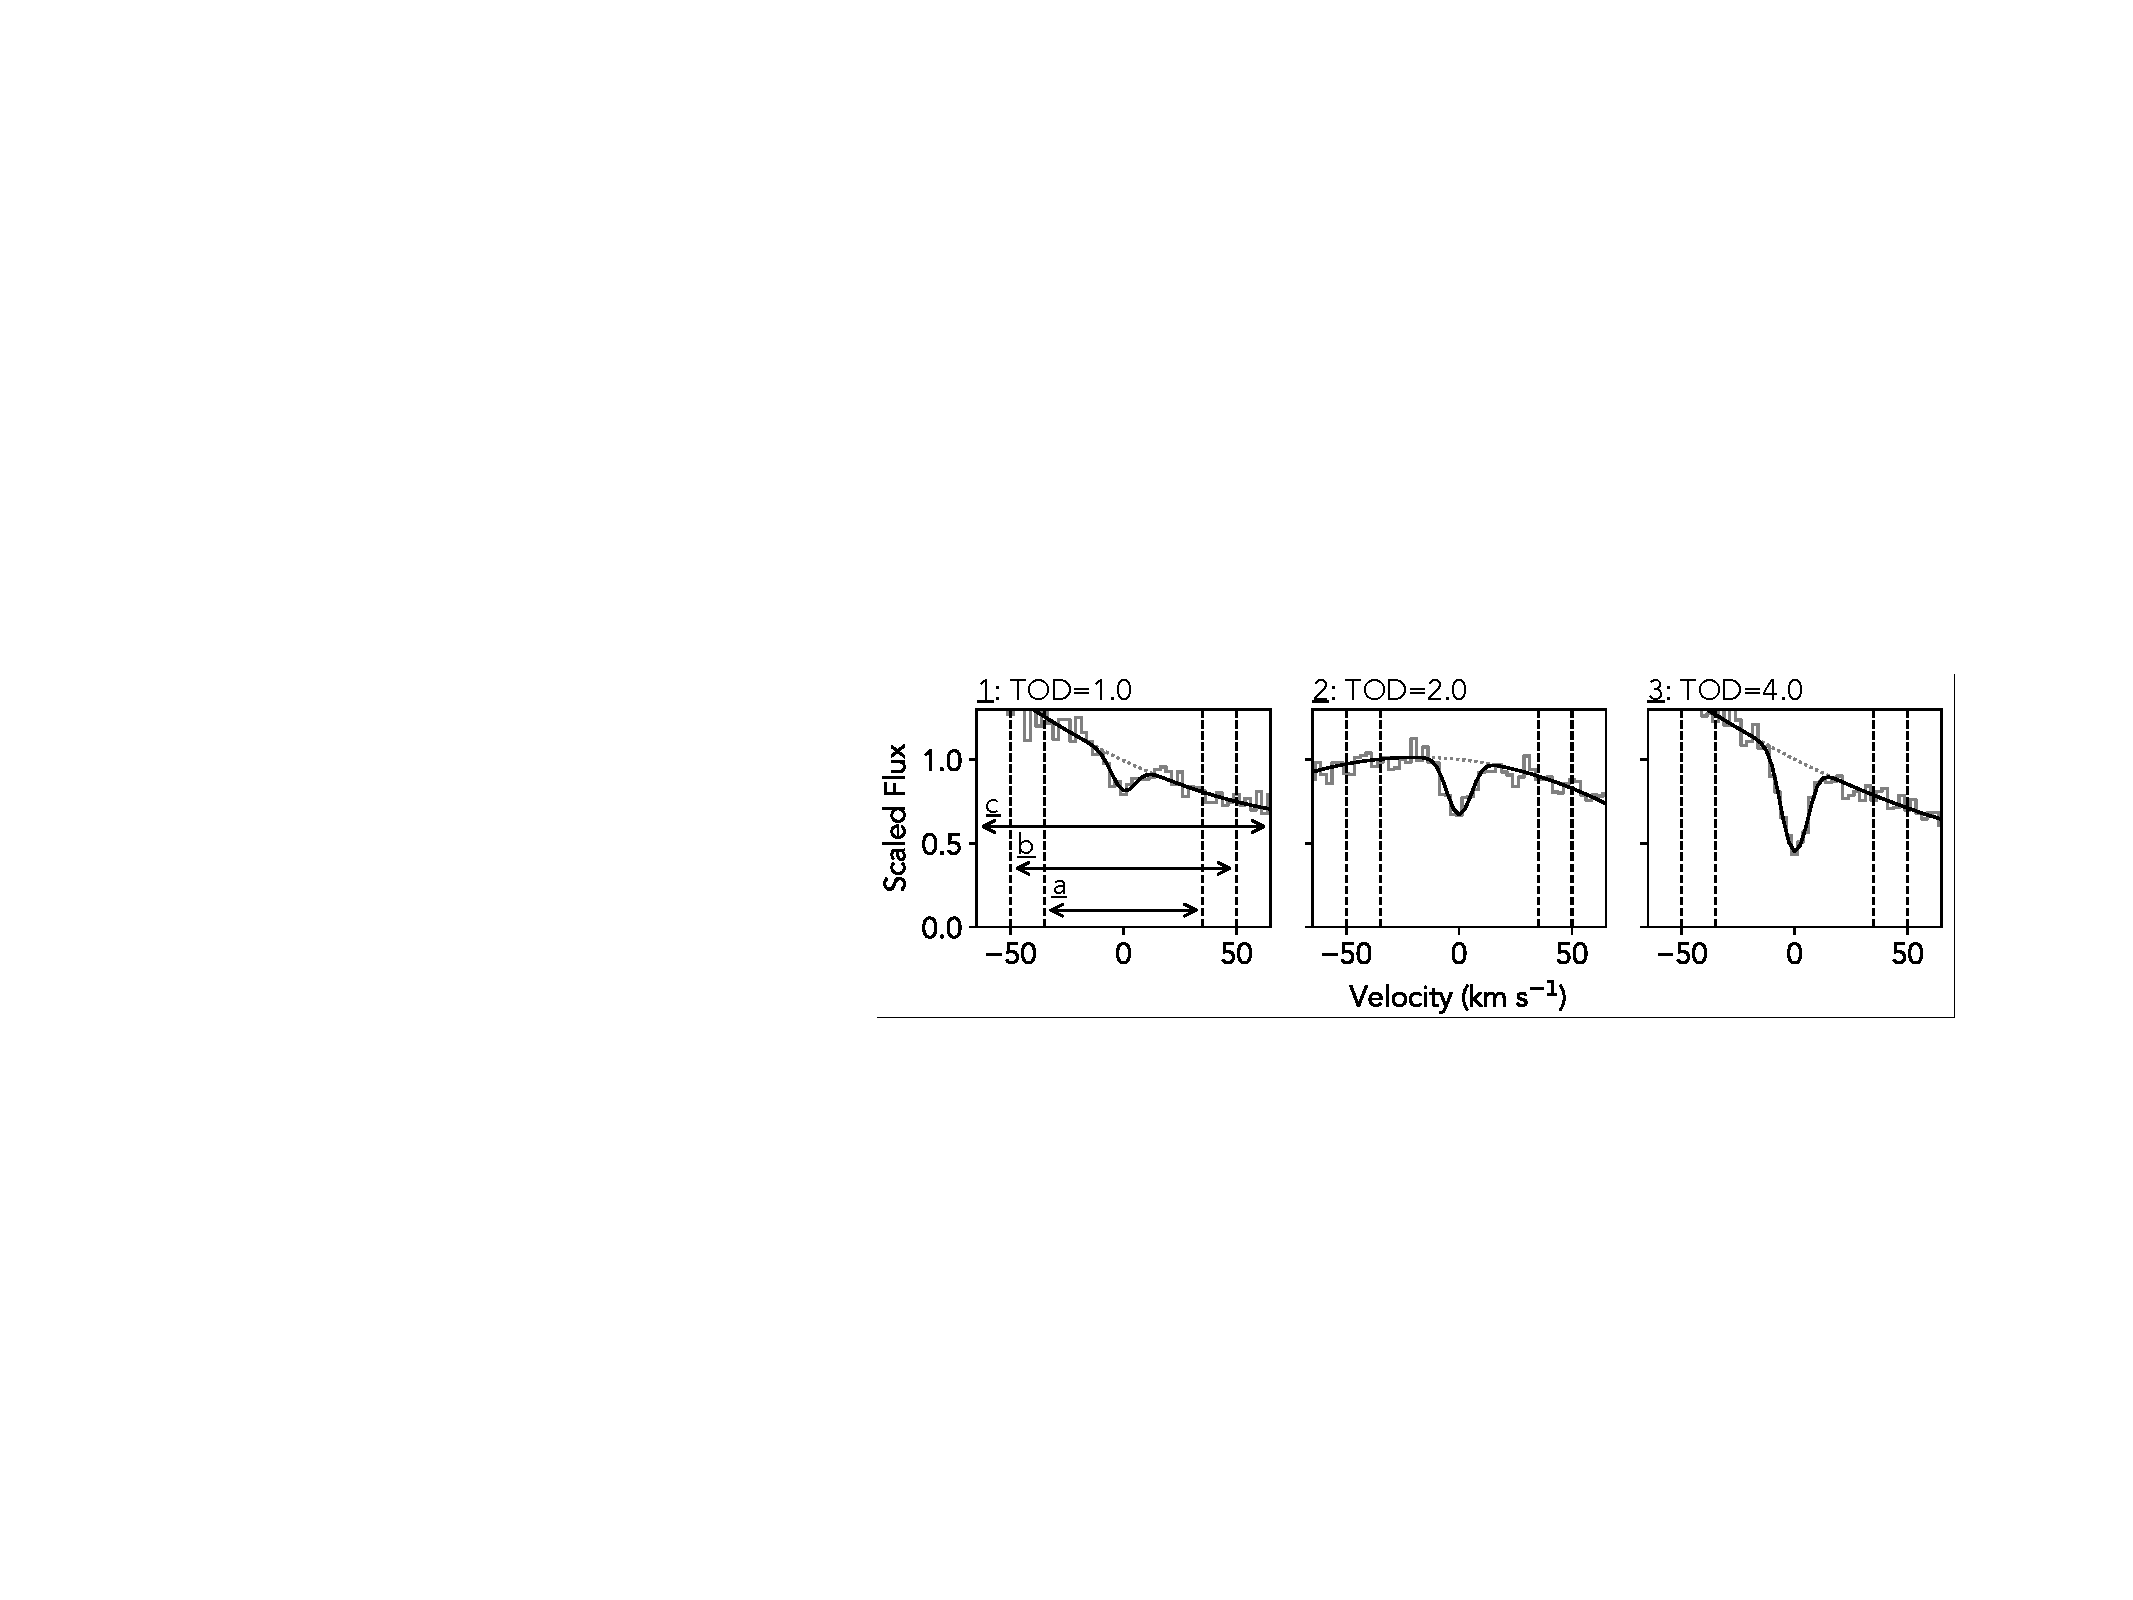
\includegraphics[width=\linewidth]{figures/annotated_example_data.pdf}
  \caption{
  \bf
  Examples of the artificial spectra that are used in the tests described in Section \ref{sec:test-cases}.
  Each panel shows a noise-free spectrum with absorption (solid black line), a noise-free continuum (dotted gray line), and a noisy realization of the spectrum with absorption (solid gray).
  These artificial spectra have a signal-to-noise ratio of 20 and a polynomial of degree 2 as the continuum.
  The panels are numbered in order of increasing total optical depth (TOD).
  The vertical lines and letters shown in each panel correspond to different spectrum extents, $\pm 35$ (a), $\pm 50$ (b), and $\pm 65$ km s$^{-1}$ (c).
  The numbers and letters used to indicate TODs and spectrum extents in this figure are consistent with the labeling used in Figures \ref{fig:outcomes-CO-1} and \ref{fig:outcomes-CO-2}.
  }
  \label{fig:artificial-data-eg}
\end{figure}

{ \bf
In this section, we explore how different continuum placement methods affect the accuracy and precision with which column densities can be measured from absorption lines.
We do this by generating artificial spectra containing absorption lines with known input parameters and measuring line parameters using different continuum placement methods.
The central question of this section is: \emph{Are line parameters obtained while marginalizing over continuum parameters more accurate and precise than line parameters obtained while using other continuum placement strategies?}
The answer depends on whether or not a correct, informative prior over continuum parameters is used for marginalization.
If an informative and accurate prior is available, continuum marginalization produces results that are almost as precise and accurate as those obtained using the continuum actually used to generate the spectrum.
If continuum marginalization is instead done with a diffuse, uninformative prior, the results are no better than simultaneously fitting for line and continuum parameters.

To isolate the effect of continuum placement, we keep the test problem simple: a single resolved and unsaturated absorption line superimposed on a continuum that is a first or second degree polynomial (i.e. a line or a quadratic function).
We vary the depth of the absorption line, the extent of the spectrum surrounding the line, and the signal-to-noise ratio (SNR) of the artificial data.
We generate 2000 spectra for each combination of total optical depth, SNR, spectrum extent, and continuum degree.
Each spectrum has a different set of continuum parameters, which are generated from a normal distribution.
The input parameters we adopt are listed in Table \ref{tab:artificial-data:params}.
Example spectra generated using each of the considered total optical depths and extents are shown in Figure \ref{fig:artificial-data-eg}.
}

{ \bf
\subsection{Continuum placement methods}
\label{sec:artificial-tests:continuum-placement-methods}
We consider two categories of continuum placement method: ones in which continuum parameters are optimized for, or \emph{fitted continuum (FC) methods}, and ones in which continuum parameters are marginalized over, or \emph{marginalized continuum (MC) methods}.
We also consider a case where the true continuum is known (case TC) and only the line parameters need to be determined.
Since case TC's error in line parameters due to continuum placement error is, by definition, identically zero, case TC provides an estimate of the error purely due to independent normally-distributed noise.
To determine line parameters from a spectrum in case TC, we minimize\footnote{All optimization done using routines from the \texttt{SciPy} package's \texttt{optimize} module.} the discrepancy between the data and a model consisting of the correct continuum attenuated by an absorption line.

Within the two categories, we define methods based on different amounts of prior knowledge about the continuum.
In the continuum fitting category, we provide two levels of prior knowledge: knowledge of which part of the spectrum is effectively free of absorption and no additional knowledge besides which continuum parametrization to use (i.e. whether to use a first or second degree polynomial).
The first level represents a perfectly competent analyst or algorithm selecting an absorption-free region over which to fit a continuum.
The second level provides enough information to ensure that the correct solution is allowed by the model.
To determine line parameters given a true absorption-free region, we fit a continuum to this region and then optimize for line parameters assuming the obtained continuum.
To determine line parameters just given the correct continuum parameterization, we simultaneously optimize for continuum and line parameters.
We will refer to these continuum placement methods by the abbreviations TR-FC (True Region-Fit Continuum), and FC (Fit Continuum).

We provide three levels of prior knowledge in the continuum marginalization category: knowledge of the correct prior; knowledge of several possible priors, one of which is the correct prior; and no meaningful prior knowledge.
The correct prior is the distribution used to generate the continuum parameters.
This level of knowledge provides a baseline for how well it is possible to recover absorption line parameters while using continuum marginalization.
The second level can be thought of as having accurate knowledge of the range of plausible continuum shapes in several distinct classes of continuum, but not knowing in advance which class should be used for a given spectrum.
The third level is a pessimistic scenario and is analogous to method FC.
To ensure numerical stability, we still use a proper prior in this method, but one which is orders of magnitude broader than the correct one.
In the first and third methods, absorption line fitting is done using the logarithm of Equation \ref{eqn:proper-prior-marginal} as the objective function.
In the second method, the objective function is the logarithm of Equation \ref{eqn:parametrization-marginalization}.
We refer to these continuum placement methods by the abbreviations TCov-MC (True Covariance-Marginalized Continuum), MCov-MC (Marginalized Covariance-Marginalized Continuum), and DCov-MC (Diffuse Covariance-Marginalized Continuum).

}

{ \bf
\subsection{Results and Discussion}

\begin{figure}
  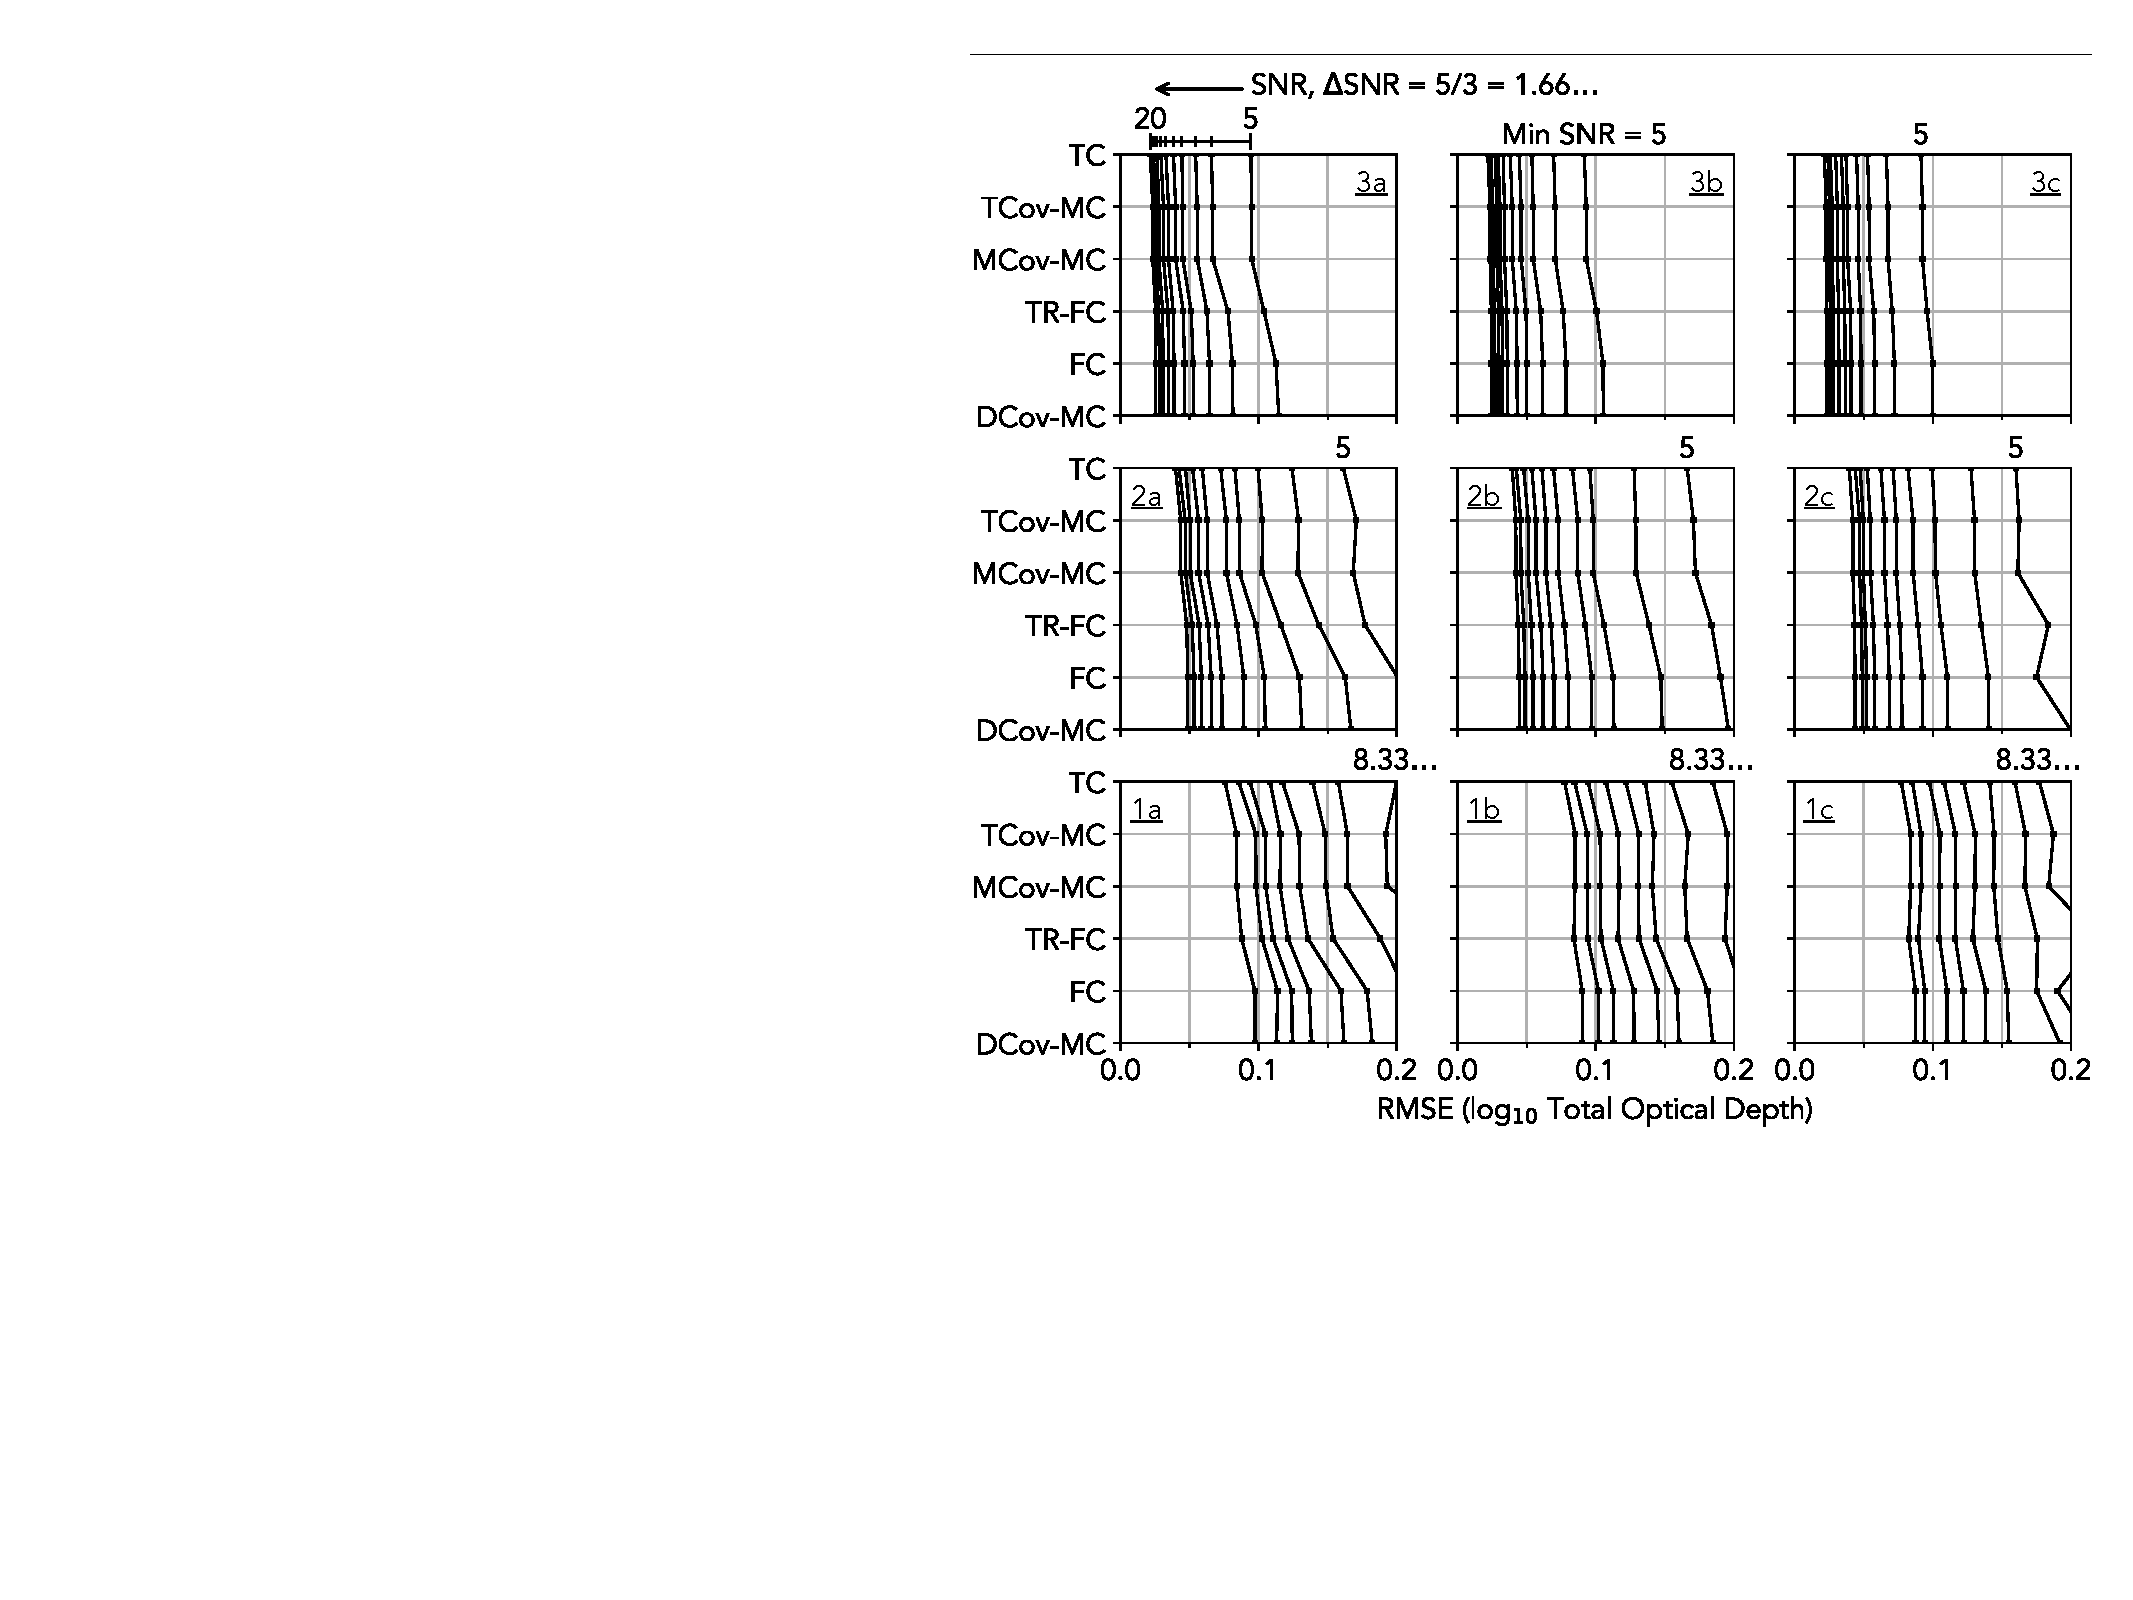
\includegraphics[width=\linewidth]{figures/annotated_co1_RMSEs_vs_SNR.pdf}
  \caption{
  \bf
  How the root mean square error (RMSE) in the recovered log total optical depth (TOD) varies as a result of changing the true TOD of the absorption feature, the extent of the spectrum around the absorption feature, the signal-to-noise ratio (SNR) of the spectrum, and the continuum placement method.
  In this figure, the continuum is a polynomial of degree 1, i.e. a line.
  Each panel corresponds to a different combination of true TOD and spectrum extent.
  The TOD increases from bottom to top and is indexed by the underlined number in the corner of each panel; the indices 1, 2, and 3 correspond to the linear (i.e. non-log) TODs of 1.0, 2.0, and 4.0. The spectrum extent increases from left to right and is indexed by the underlined letter in the corner of each pixel; the indices a, b, and c correspond to extents of $\pm 35$, $\pm 50$, and $\pm 65$ km s$^{-1}$. These labels are consistent with those used in Figure \ref{fig:artificial-data-eg}, which shows examples of spectra at each combination of TOD and spectral extent.
  Within each panel, each line connecting a series of points corresponds to a different SNR; these are labeled at the top of panel 3a. The minimum SNR whose RMSEs are small enough to fall within the range shown is indicated at the top of each panel.
  The vertical axis within each panel corresponds to different continuum placement methods. The full names corresponding to the abbreviations shown here are given in Section \ref{sec:artificial-tests:continuum-placement-methods}.
  }
  \label{fig:outcomes-CO-1}
\end{figure}

\begin{figure}
  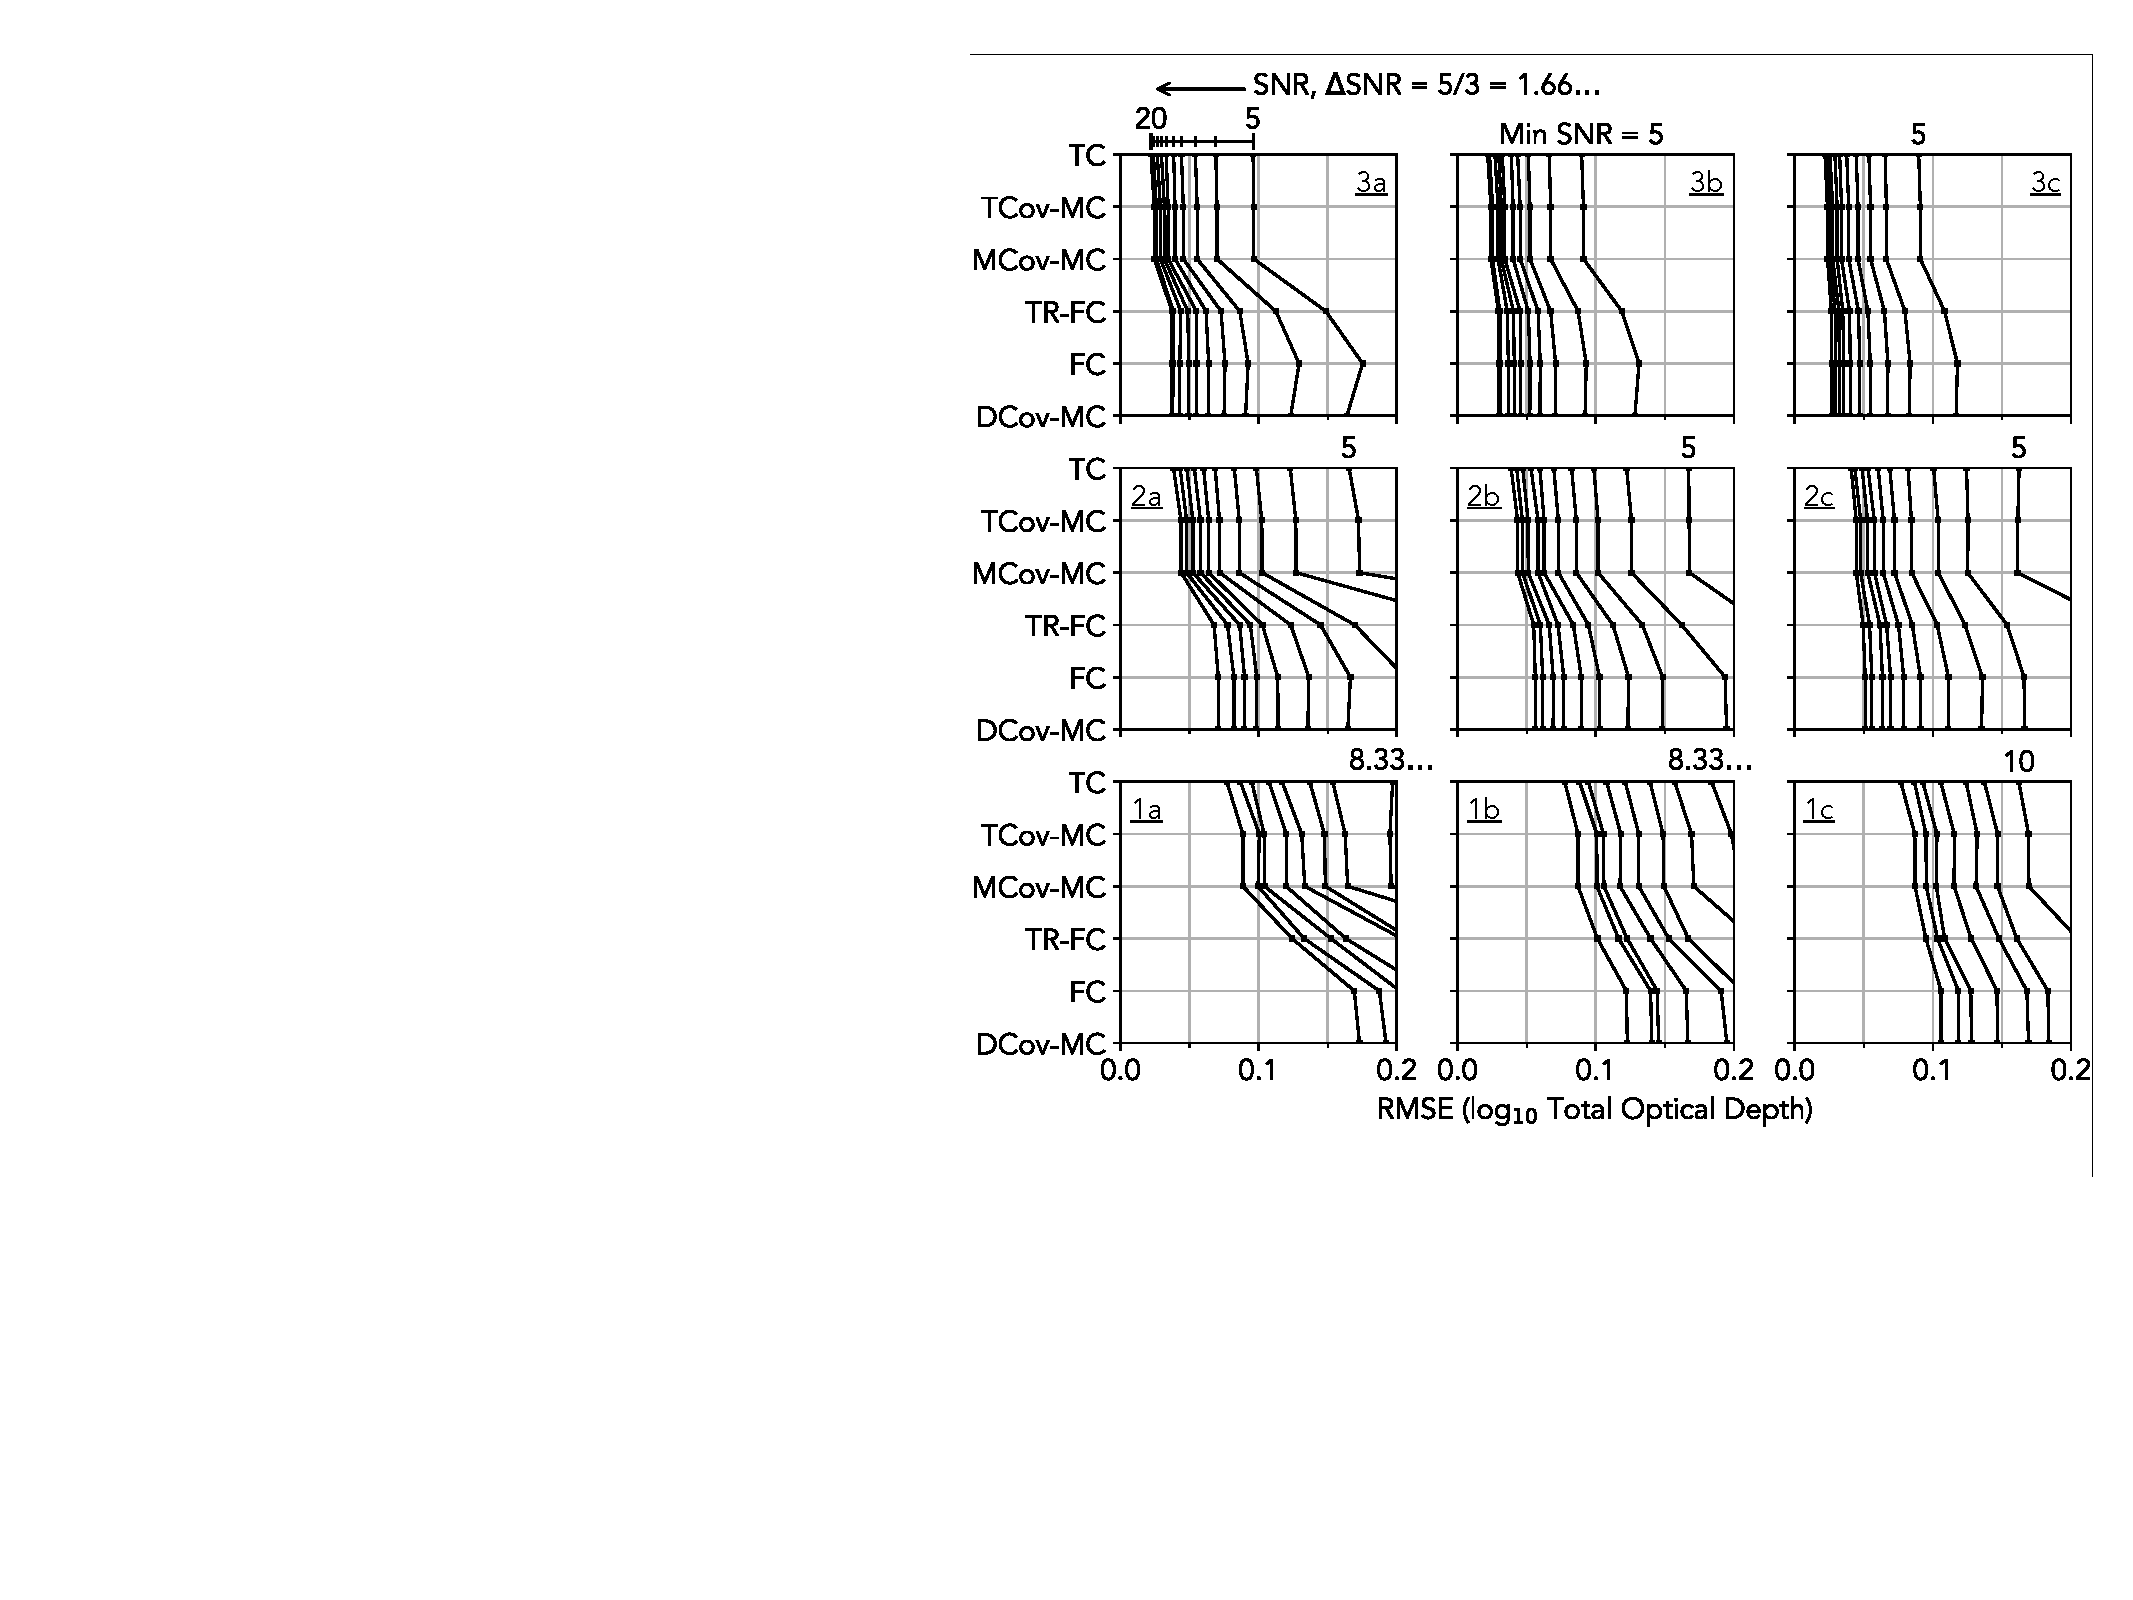
\includegraphics[width=\linewidth]{figures/annotated_co2_RMSEs_vs_SNR.pdf}
  \caption{
  \bf
  How the root mean square error (RMSE) in the recovered log total optical depth (TOD) varies as a result of changing the true TOD of the absorption feature, the extent of the spectrum around the absorption feature, the signal-to-noise ratio (SNR) of the spectrum, and the continuum placement method.
  In this figure, the continuum is a polynomial of degree 2, i.e. is a quadratic function.
  Panel labels and axes are defined in the caption to Figure \ref{fig:outcomes-CO-1}.
  }
  \label{fig:outcomes-CO-2}
\end{figure}

\begin{figure}
  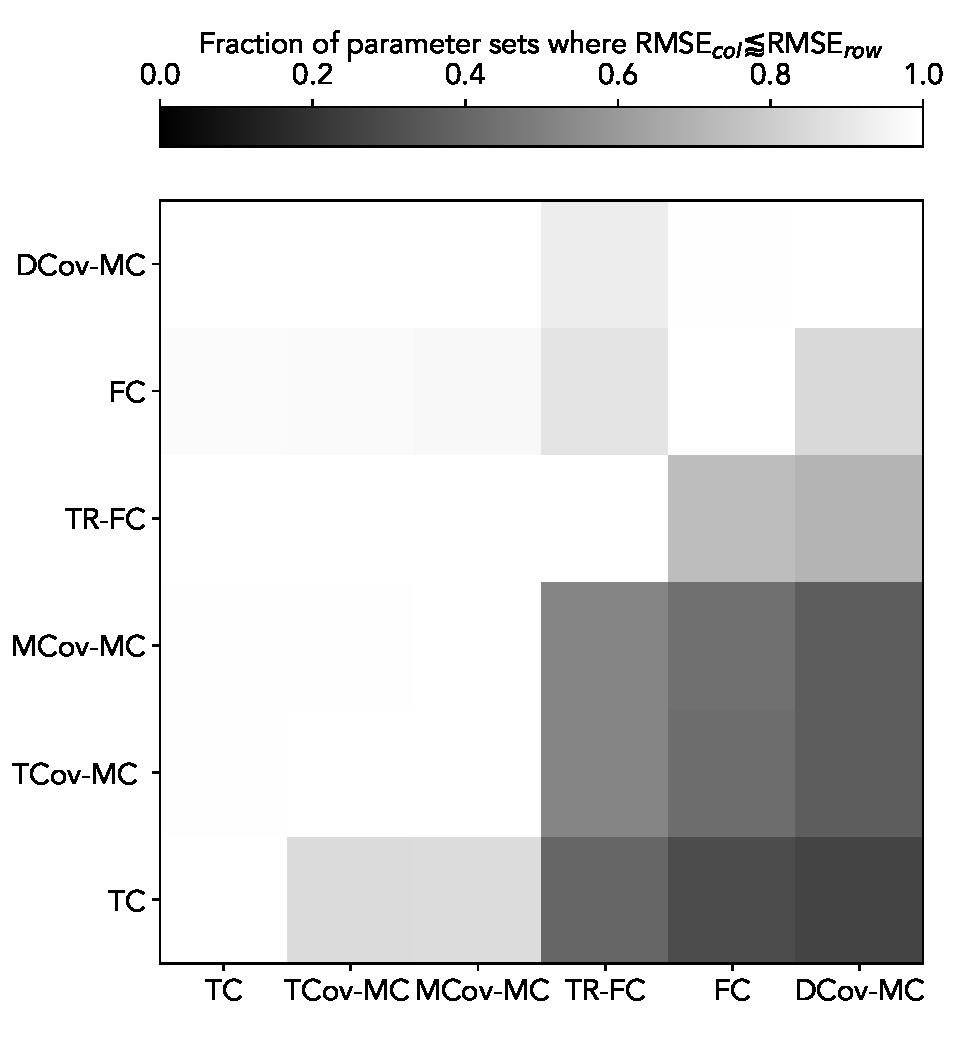
\includegraphics[width=\linewidth]{figures/overall-performance.pdf}
  \caption{
  \bf
  A summarized comparison of the relative performance of different continuum placement methods.
  Each row and each column corresponds to a different method.
  The method names corresponding to the abbreviations are given in Section \ref{sec:artificial-tests:continuum-placement-methods}.
  The color of each pixel indicates the fraction of input parameter sets for which the log total optical depth (TOD) root mean square error (RMSE) of the method on the $x$-axis is less than or within 0.01 dex of the log TOD RMSE of the method on the $y$-axis.
  This comparison quantity is an average across the different continuum degrees, true TODs, and spectrum extents and signal-to-noise ratios.
  The higher the fraction is, the better---a value of 1.0 means the method on the $x$-axis is at least as precise/accurate as the method on the $y$-axis for every input parameter set.
  }
  \label{fig:outcomes-summary}
\end{figure}
Using these six objective functions and non-linear optimization routines from the \texttt{SciPy} package, we fit absorption profiles to each of the generated test spectra.
This yields one set of line parameters---center, breadth, and total optical depth---per test spectrum.
Because it is the most challenging line parameter to correctly recover, we will focus on the total optical depth.
To quantify quality of recovery, we compute the root mean square error (RMSE) of the logarithm of the total optical depth:
\begin{equation}
  \label{eqn:RMSE-def}
  RMSE(\log\tau) = \sqrt{
    \frac{1}{N} \sum_{i=1}^{N} \left( \log\hat{\tau}_i - \log\tau_{\rm true} \right)^2
  }.
\end{equation}
$\hat{\tau}_i$ is the total optical depth value recovered from spectrum realization $i$ and $\tau_{\rm input}$ is the total optical depth actually used to generate the spectra.
We use the RMSE of the logarithm instead of the linear value of the total optical depth because it is equal to the RMSE of a corresponding column density.
The total optical depth of a line is equal to the product of the column density of the absorber and some physical constants.
The difference of the logarithms of a pair of total optical depths is therefore equal to the difference of the logarithms of the corresponding column densities---the multiplicative constant factors become additive and cancel.

The RMSEs for each combination of input parameter set and continuum placement method are shown in Figures \ref{fig:outcomes-CO-1} and \ref{fig:outcomes-CO-2}.
One way to summarize these results across the tested parameter space is to compare the performance of each method relative to the performance of each other method.
To do this quantitatively, we calculate the fraction of cases in which the RMSE of method A is less than or equal to the RMSE of method B.
A visual representation of this relative performance summary is shown in Figure \ref{fig:outcomes-summary}.

The two informed continuum marginalization methods, TCov-MC and MCov-MC, consistently yield the lowest RMSEs of all the continuum placement methods.
For about 80\% of the fixed input parameter combinations, TCov-MC and MCov-MC perform as well as the known-continuum reference case, TC.
Informed continuum fitting, TR-FC, performs more poorly than informed marginalization but better than both uninformed fitting and uninformed marginalization.
Finally, uninformed fitting, FC, performs better on average than uninformed marginalization, DCov-MC.

\emph{The value of different kinds of prior continuum information.}
The different methods combine prior and observed continuum information.
The performance of the methods reflects the value of the prior information available to them and the efficiency with which they extract continuum information from the observed spectrum.

By definition, case TC has as much continuum information as it is possible to have.
The fact that methods TCov-MC and MCov-MC perform almost as well as case TC suggests that the accurate priors used in these methods are almost as informative as knowing the actual continuum.
These particular priors are not so constraining that all continuum realizations would be indistinguishable.
The (clearly distinguishable) continua of the spectra shown in Figure \ref{fig:artificial-data-eg} were generated from the prior used in method TCov-MC.
The prior used by method MCov-MC is less specific, but apparently no worse, than that of TCov-MC.
The fact that these priors are so informative is noteworthy because it is, in many cases, possible to infer them; this point is discussed further in Section REFTKTK.

The performance of method TR-FC suggests that knowing where the spectrum is free of absorption has value, but not as much as an accurate prior on the continuum shape.
The value of this information is greatest for parameter sets with the lowest TOD, i.e. the least contrast between the continuum and absorption.

\emph{Solutions with RMSEs that are lower than those of the TC solution are biased.}
There is a small number of fixed input parameter combinations for which the RMSE of method FC is lower than that of case TC.
All of these combinations have low SNRs, small TODs, and short continuum extents.
This can be explained by the fact that much of the RMSE of method FC for these combinations is due to bias, rather than variance.
Method FC is consistently finding solutions that are incorrect by an amount that is small relative to the scatter in the less-biased TC solution.
This bias is favorable for those particular true line parameters, but may be unfavorable for other values of the true line parameters.

\emph{Continuum marginalization is not substantially slower than continuum fitting.}
On a single core of a 2.2 GHz Intel i7 processor, obtaining line parameters for 2000 spectra took approximately 2 seconds in case TC, 5 seconds with method TR-FC, 10 seconds with methods MCov-MC and DCov-MC, 15 seconds with method FC, and 20 seconds with method MCov-MC.
Method TR-FC is a factor of 2-4 as fast as the other continuum placement methods once absorption is masked.
When analyzing actual observations, this advantage would be outweighted by the human interaction time required to define absorption masks.
}


\section{A Demonstration on Actual Data}

\begin{figure}
  \centering
  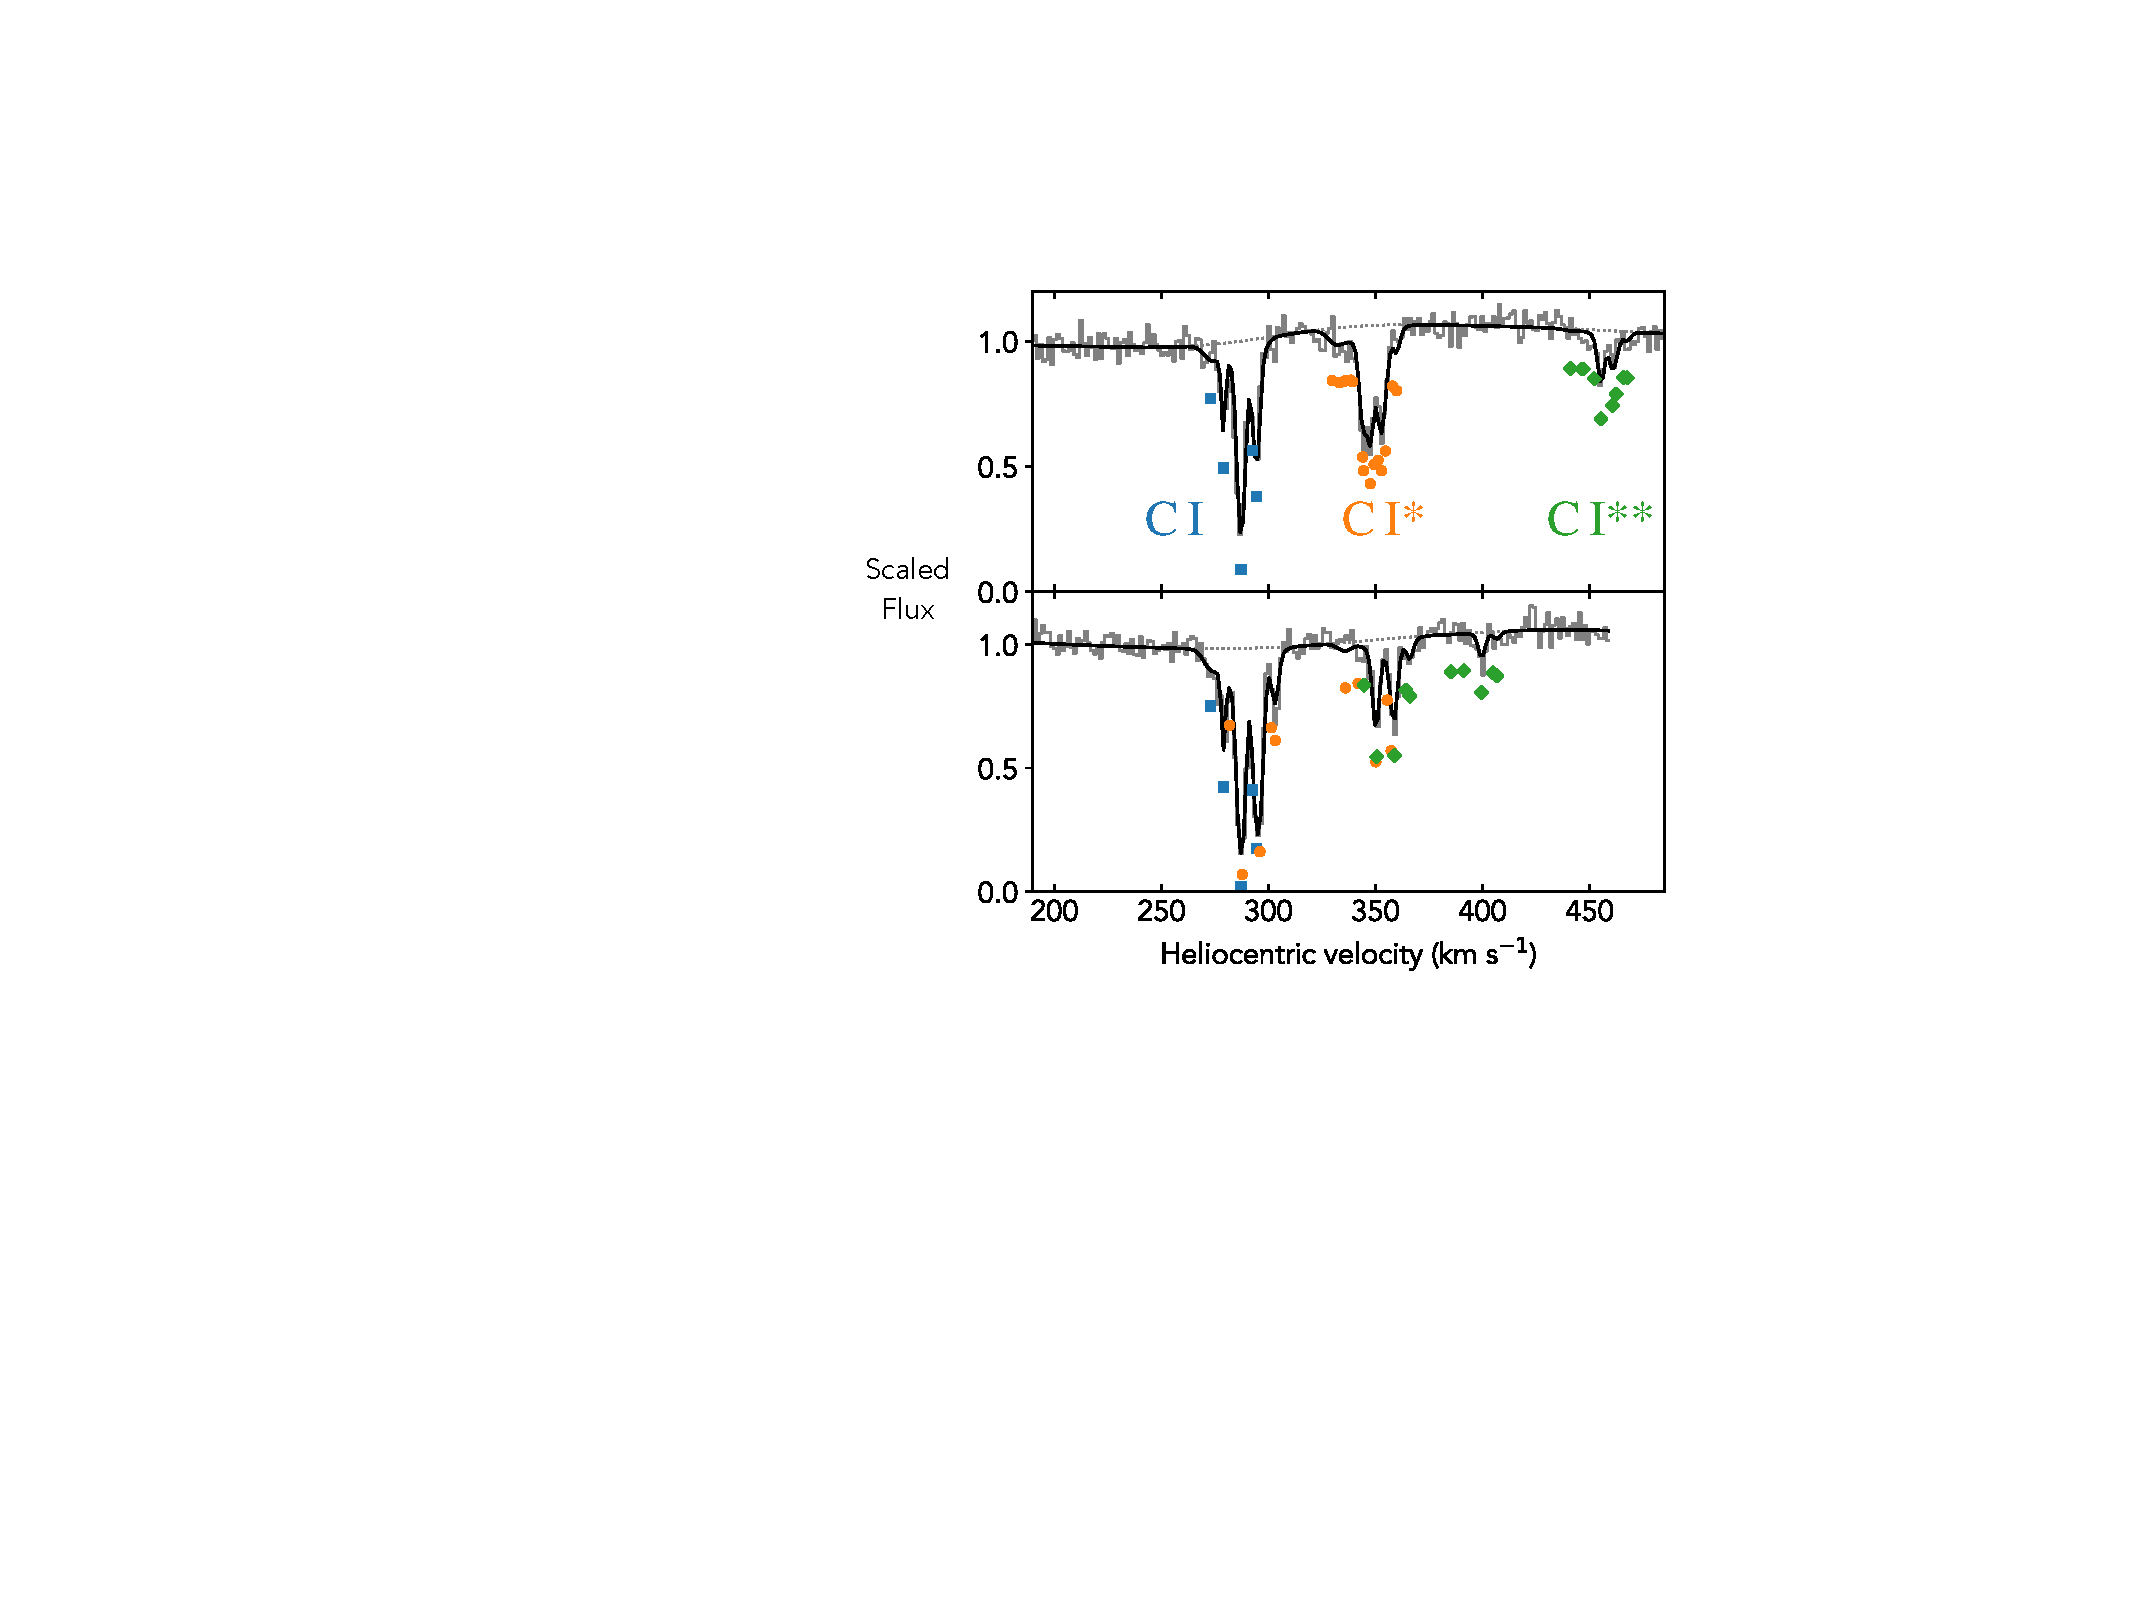
\includegraphics{annotated-SK-675.pdf}
  \caption{
  A fit to absorption from ground and excited state {C \small{I}} absorption towards the star Sk-67 5 in the Large Magellanic Cloud.
  The data, continuum, and combined fit are shown in solid gray, dotted gray, and solid black lines.
  The velocities shown on the $x$-axis are relative to the {C \small{I}} $\lambda$1329\AA{} (top panel) and $\lambda$1277\AA{} lines (bottom panel).
  Line centers of the ground and first two excited states are indicated by datapoints of different shapes and colors.
  The number of excited state line centers is greater than the number of ground state line centers because there are multiple excited state transitions and a single ground state transition in each velocity range.
  }
  \label{fig:demonstration-fit}
\end{figure}

{ \bf
In this section, we analyze absorption features in using continuum marginalization in a case where all continuum placement methods should agree.
The absorption features are due to {C \small{I}} in the Large Magellanic Cloud (LMC).
The data are spectra of the LMC stars Sk-67 5, Sk-68 73, and Sk-70 115 taken with the Space Telescope Imaging Spectrograph (STIS) \citep{1998PASP..110.1183W} on board the \emph{Hubble Space Telescope} (\emph{HST}) using the E140H grating ($R \sim 114,000$).
We adopt the {C \small{I}} column density measurements of \citet{Welty:2016} as ground truth.
\citet{Welty:2016} used fitting to manually selected line-free regions to determine the continuum.

We downloaded the default pipeline-extracted one-dimensional spectra from the Mikulski Archive for Space Telescopes (MAST).
Individual exposures within a single echelle order were shifted using nearest neighbor interpolation to the wavelength grid of one of the exposures and coadded.
We did not splice different echelle orders into a combined spectrum.

To measure {C \small{I}} column densities, we fit Voigt profiles to the {C \small{I}}, C\small{I}$^*$, and C\small{I}$^**$ absorption in these spectra.
The model we used for the continuum was the sum of a first degree polynomial and a Gaussian process with a Matern-5/2 kernel.
The LSFs we used were downloaded from the \emph{HST}-STIS website\footnote{\url{http://www.stsci.edu/hst/instrumentation/stis/performance/spectral-resolution}.}
Following the example of \citet{Welty:2016}, we analyzed only the {C \small{I}} multiplets near 1280.1\AA and 1328.8\AA.
All absorption features for a target were fit simultaneously by maximizing the continuum-marginalized likelihood function of the data given the absorption model.
Each velocity component had a single central velocity and breadth and a separate column density for the ground and two excited states of {C \small{I}}.
Optimizing over the profile parameters while marginalizing over continuum parameters for a single object took between a few and 10 seconds per target.
The computation time is dominated by evaluating the continuum-marginalized likelihood and its gradient with respect to the Voigt profile parameters.

The maximum likelihood absorption solution for target Sk-67 5 is shown in Figure \ref{fig:demonstration-fit}.
For all three targets, the total recovered {C \small{I}} column densities across all velocity components and excitation levels agree within the uncertainties with those found in \citet{Welty:2016}.
The agreement is expected, given that these are data with high spectral resolution and SNR and the absorption lines are narrow and clearly distinct from the continuum---all valid continuum placement methods should yield the same result.

We have chosen a dataset with these characteristics to limit the plausible reasons for any potential disagreement to the continuum placement method.
Preparing a more challenging low SNR spectrum for analysis often requires bespoke, and proprietary, processing (see e.g. \citealt{Wakker:2015} for a well-documented example).
As a result, there is no guarantee that there should be agreement between line parameters obtained using the same continuum placement and line fitting method applied to different reductions.
To be able to compare results produced by continuum marginalization against the best efforts of other analysts, we therefore chose a dataset where there should be no such ambiguity.
}


\section{Discussion}
\label{sec:discussion}
\subsection{Assumptions and consequences}
{\bf
The explicit assumptions of the analytic marginalization method are that the continuum is a linear combination of basis functions, that the prior on the coefficients of this linear combination is the improper uniform or multivariate normal distribution, that residuals between the data and model are normally distributed, and that the covariance matrix of the residuals does not depend on the continuum.
It is obvious that these assumptions do not hold in a strict sense for any dataset.
For example, both possible priors require that there not be constraints on the coefficients, meaning that negative continuum values must be allowed even though no background source produces negative flux.
In practice, models with negative fluxes will be poor descriptions of any real dataset and will contribute little posterior probability mass.
This issue is also not unique to continuum marginalization, analytic or not.
Describing residuals with a normal distribution, as is conventionally done with spectra given in continuous rate units such as flux, allows negative models values.
}

{\bf
A less trivial example are data in the low photon count regime.
Depending on whether a spectrum is left in terms of photons or converted to a rate (or further transformed into e.g. a flux) and on whether and how background subtraction is done, the value of a low photon count measurement is best described by a Poisson, Skellam, Gamma, or difference-of-Gammas distribution.
All of these distributions converge to the normal distribution as the number of photons grows, but are poorly approximated by it at low counts.
Furthermore, the variance of these distributions depends on the count rate, meaning that the uncertainty of the measurement depends on the true value of the measurement.
This means that at low counts, point estimates of the uncertainties, such as those produced by spectral extraction pipelines, will themselves be uncertain.
Errors in the uncertainty of the measurement will be covariant with errors in the measurement itself.
It is therefore best to work with the appropriate distribution rather than with the uncertainty point estimate and the normal approximation.
}
This means that analytic marginalization of the kind described in this work should not be applied to low SNR X-ray or UV spectra.

Another assumption of the method that can be non-trivially broken is that the absorption model is realistic.
For analytic marginalization to be useful, it must be possible for the absorption model to correctly describe the actually present absorption features.
For example, if a region of a spectrum contains two clearly distinct absorption lines but the model only allows for a single line, the presence of the un-modeled line can bias the continuum model.
In short, improvements in continuum modeling cannot solve problems of absorption model misspecification.


The continuum models envisaged in this work will usually be effective descriptions rather than (often non-linear) physical descriptions.
{ \bf The continua of most background sources that are used for absorption spectroscopy can be approximated in this way.}
Examples of sources with slowly varying continua include quasars and (particularly rapidly rotating) hot stars.
With flexible linear models such as splines, it is even possible to describe more complicated pseudo-continua such as stellar wind lines.
For even more complicated pseudo-continua such as those of cool stars \citep[e.g.]{Zasowski:2015hi}, it is necessary to use a non-linear model.
Marginalizable linear models can still be useful even in this case as a way of introducing small corrections for pseudo-continuum features that are not perfectly described by the non-linear model.


{
\subsection{Informative priors are valuable and realistically obtainable}
+ remind reader that I've shown that having an informative prior can be almost as good as knowing the true continuum

- this is interesting because while getting access to the true continuum is not possible in an absolute sense, it is in many cases possible to get an informative prior.
- two straightforward cases are coherent classes of background sources and \emph{stationarity} of continuum of a single background source.

- certain kinds of background sources make up a coherent class with continua whose variation from source to source can be accurately described with a small number of free parameters.
- one such class is Type TKTK quasars.
- large samples of quasar spectra have been used to derive sets of basis functions that capture how the quasar continuum shape varies across the class EG TKTK.
- This is, first of all, actually already a prior.
- supplementing it with a prior on the amplitudes of coefficients or even the covariances of the coefficients adds further information.
- an example where a quasar-derived prior was actually used in (numerical) marginalization over quasar continua for the purpose of absorption line analysis is given in \citet{2017ApJ...844..136E}.

- other kinds of sources have continua that can be approximated by stationary stochastic processes.
- stationarity here means that the way in which the continuum varies as a function of wavelength is consistent.
- even though no piece of the continuum is necessarily the same as a different piece, each piece has similar statistical properties.
- for a concrete example, consider fitting polynomials to different regions of a spectrum.
- even though each region will have different polynomial coefficients, it is possible that coefficients have a typical amplitude.
- this typical amplitude can be learned and then used when marginalizing over the continuum in a region that also contains absorption lines.
}

\subsection{Applications of analytic marginalization}
WHOLE SECTION REWRITE
The test cases in Section \ref{sec:test-cases} showed that marginalization over continuum parameters and parameterizations is more precise, accurate, and robust than the alternatives.
Considered purely as a replacement for numerical marginalization, analytic marginalization is just a potentially more computationally efficient way of implementing an existing inference approach.
However, it also allows two qualitatively new approaches: continuum model averaging and absorption parameter optimization with a continuum-marginalized likelihood function.

The test case in Section \ref{sec:marginalization-over-parameterizations} combines both of these approaches---optimizing an absorption parameter likelihood function where the parameterization and parameters of the continuum have been marginalized over.
Analytic marginalization makes this possible in two ways: availability of closed form likelihoods and availability of gradients of closed form likelihoods.
Optimization with continuum-marginalized likelihoods is useful for analyzing large surveys.
Analyses of absorption lines in tens of thousands of spectra \citep[e.g.]{2013ApJ...770..130Z,Zasowski:2015hi} cannot practically be done with MCMC.
With analytic marginalization, it is possible to at least marginalize over continuum parameters.
The results of the test cases suggest that this approach could mean a non-trivial improvement in the accuracy and precision of absorption line measurements.

In cases where MCMC is possible, combining continuum parameterization marginalization with a probabilistic specification of absorption component structure would allow absorption line analysis with human intervention only at the level of specifying priors and candidate continuum parameterizations.
Component structure specification can be done using trans-dimensional inference, in which the dimensionality of parameter space (in this case the number of sets of absorption line parameters) is itself a parameter of the model.
This way of doing absorption line analysis has two potential advantages.
First, marginalizing over the velocity structure of the absorption as well as the continuum should automatically include effects such as unresolved saturated structure in parameter uncertainties.
TKTK TYPOS
Second, because inference approach is almost completely automatic, it allows blinding, which improves reproducibility.

\section{Conclusion}
\label{sec:conclusion}
Absorption lines are an important source of information about stars and the ISM.
As larger spectroscopic datasets become available and as reproducibility becomes more standard in astronomy, it becomes necessary to move beyond ad-hoc analysis methods, particularly ones in which a human directly interacts with data.
In multiple recent works, there have been attempts to partially automate continuum placement by including and marginalizing over continuum parameters in probabilistic spectral models.
Marginalizing over continuum parameters has, in these works, been hypothesized to also improve the accuracy of the recovered absorption line parameters.
Despite these advantages, this approach has so far not become popular, in part due to the computational expense of numerically marginalizing over these additional parameters.
- AND IN PART BECAUSE THE METHODS DIDN'T EXPLORE WHETHER OR NOT IT ACTUALLY HELPS

TKTK MAKE CHANGES
In this work, we have shown that it is possible in many cases to replace this numerical marginalization with analytic marginalization (Section \ref{sec:assumptions-and-formalism}).
Analytic marginalization speeds up MCMC-based analyses in problems with many continuum parameters (Section \ref{sec:MCMC-efficiency}).
The continuum parameter-marginalized likelihood can also be used for optimization over absorption line parameters.
This approach combines the speed of optimization with the advantages of continuum marginalization.
Analytic marginalization over continuum parameters makes it trivial to also marginalize over continuum \emph{parameterizations}.
As with parameter marginalizaton, parameterization marginalization can be combined with optimization over absorption line parameters.
Parameterization marginalization further reduces the amount of direct human interference in the analysis of individual spectra and will be especially useful in analyses of datasets containing spectra with different continuum shapes.

TKTK MAKE CHANGES
We have also confirmed that marginalization over continuum parameters and parameterizations indeed improves the accuracy of absorption line parameter measurements.
The advantage of parameter marignalization is only significant at low SNRs (Section \ref{sec:marginalization-over-parameters}).
On the other hand, parameterization marginalization is significantly more accurate than alternative methods of deciding on a continuum parameterization at all SNRs (Section \ref{sec:marginalization-over-parameterizations}).

We have released an open-source \texttt{python} package, \pkgname, which can be used to evaluate continuum parameter-marginalized likelihoods and related quantities.
Features of this package are described in Appendix \ref{sec:package-and-demos}.
It is meant to be used as a drop-in replacement for likelihood functions in existing absorption spectrum analysis tools.

\acknowledgments
The author thanks Andrew Casey, Andrew Fox, Cameron Liang, and Yong Zheng for useful discussions about use cases and Joshua Peek and Linda Tchernyshyov for helpful comments.
This research is based on observations made with the NASA/ESA Hubble Space Telescope obtained from the Space Telescope Science Institute, which is operated by the Association of Universities for Research in Astronomy, Inc., under NASA contract NAS 5–26555. These observations are associated with program TKTKTK.

\software{emcee \citep{2013PASP..125..306F},
matplotlib \citep{2007CSE.....9...90H},
numpy \citep{vanderWalt:dp},
scipy \citep{SciPy}
}

\appendix

{ \bf
\section{Convergence and effective sample generation rate of MCMC}
\label{sec:MCMC-efficiency}

\begin{figure}
  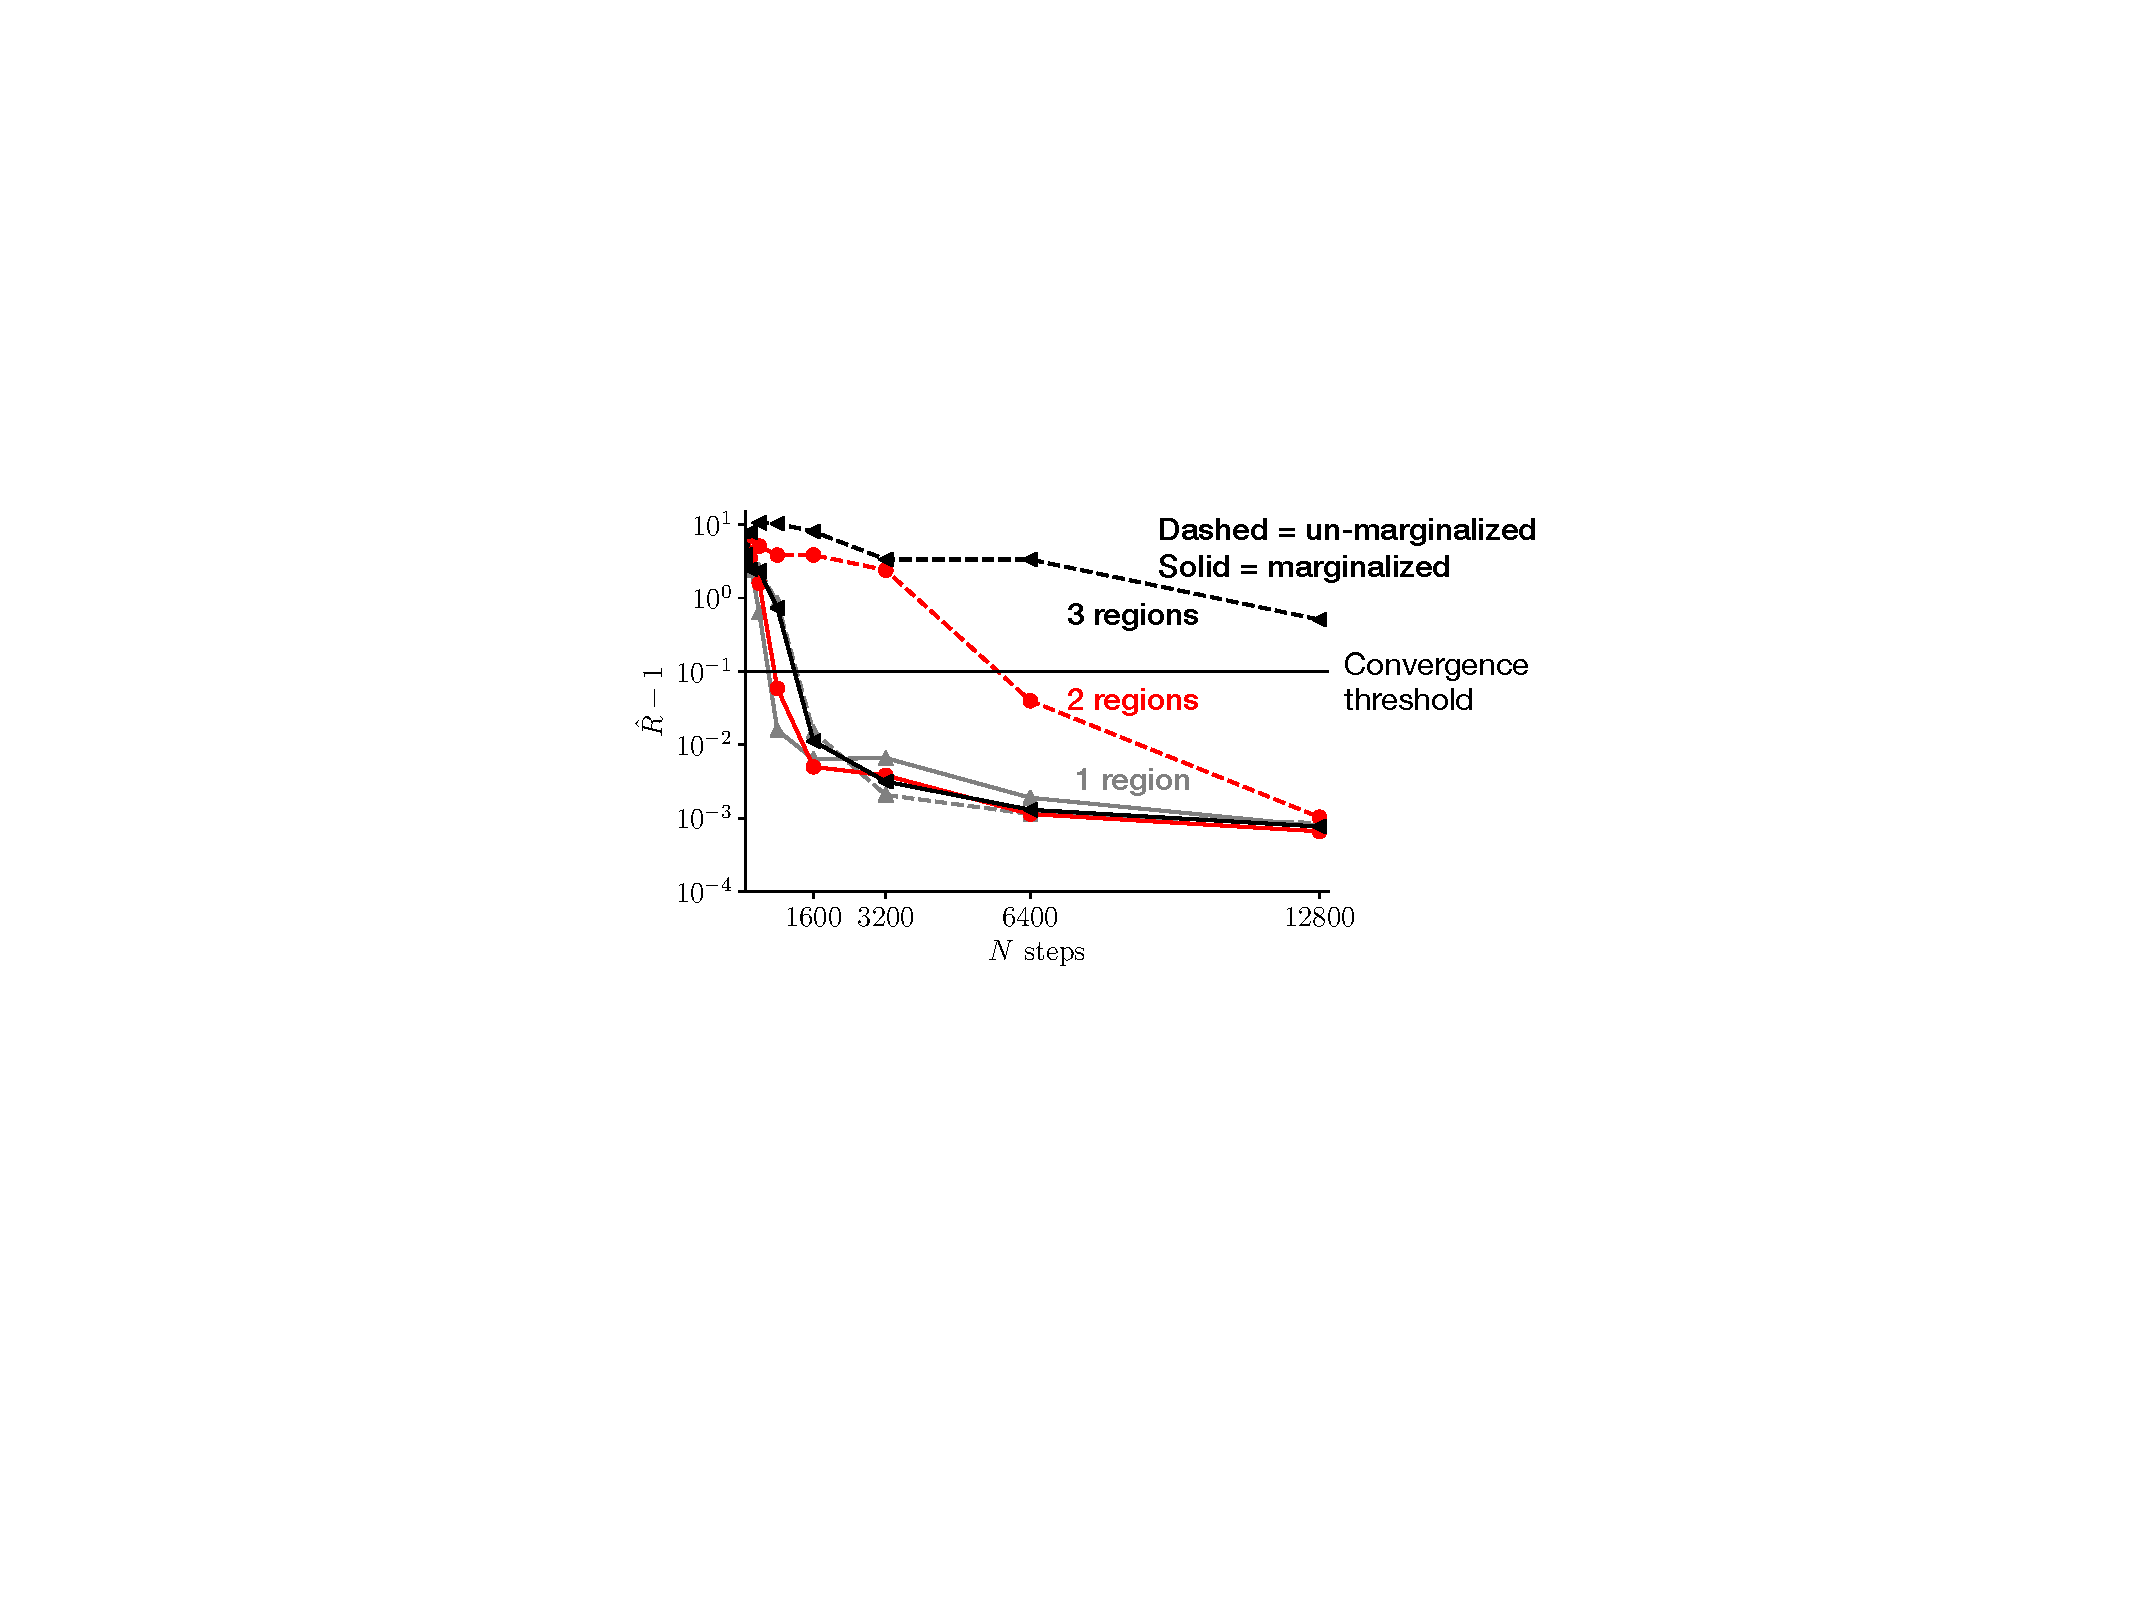
\includegraphics{convergence.pdf}
  \caption{
  Convergence rate of MCMC with analytic and numerical continuum parameter marginalization for absorption line analysis problems with different complexities.
  The convergence diagnostic (y-axis) is the Rubin-Gelman statistic, an estimate of how much smaller the Monte Carlo error of an MCMC-based parameter estimate can get.
  Each line shows the evolution of this convergence diagnostic as a function of the number of MCMC steps taken (x-axis).
  Line styles indicates whether continuum parameters are marginalized over analytically (solid) or included in MCMC (dashed).
  Line colors and markers indicate the number of spectral regions being analyzed simultaneously; each region has its own set of continuum parameters.
  The Rubin-Gelman statistic and the problem setup are discussed in more detail in Section \ref{sec:MCMC-efficiency}.
  }
  \label{fig:convergence-comparison}
\end{figure}

\begin{figure}
  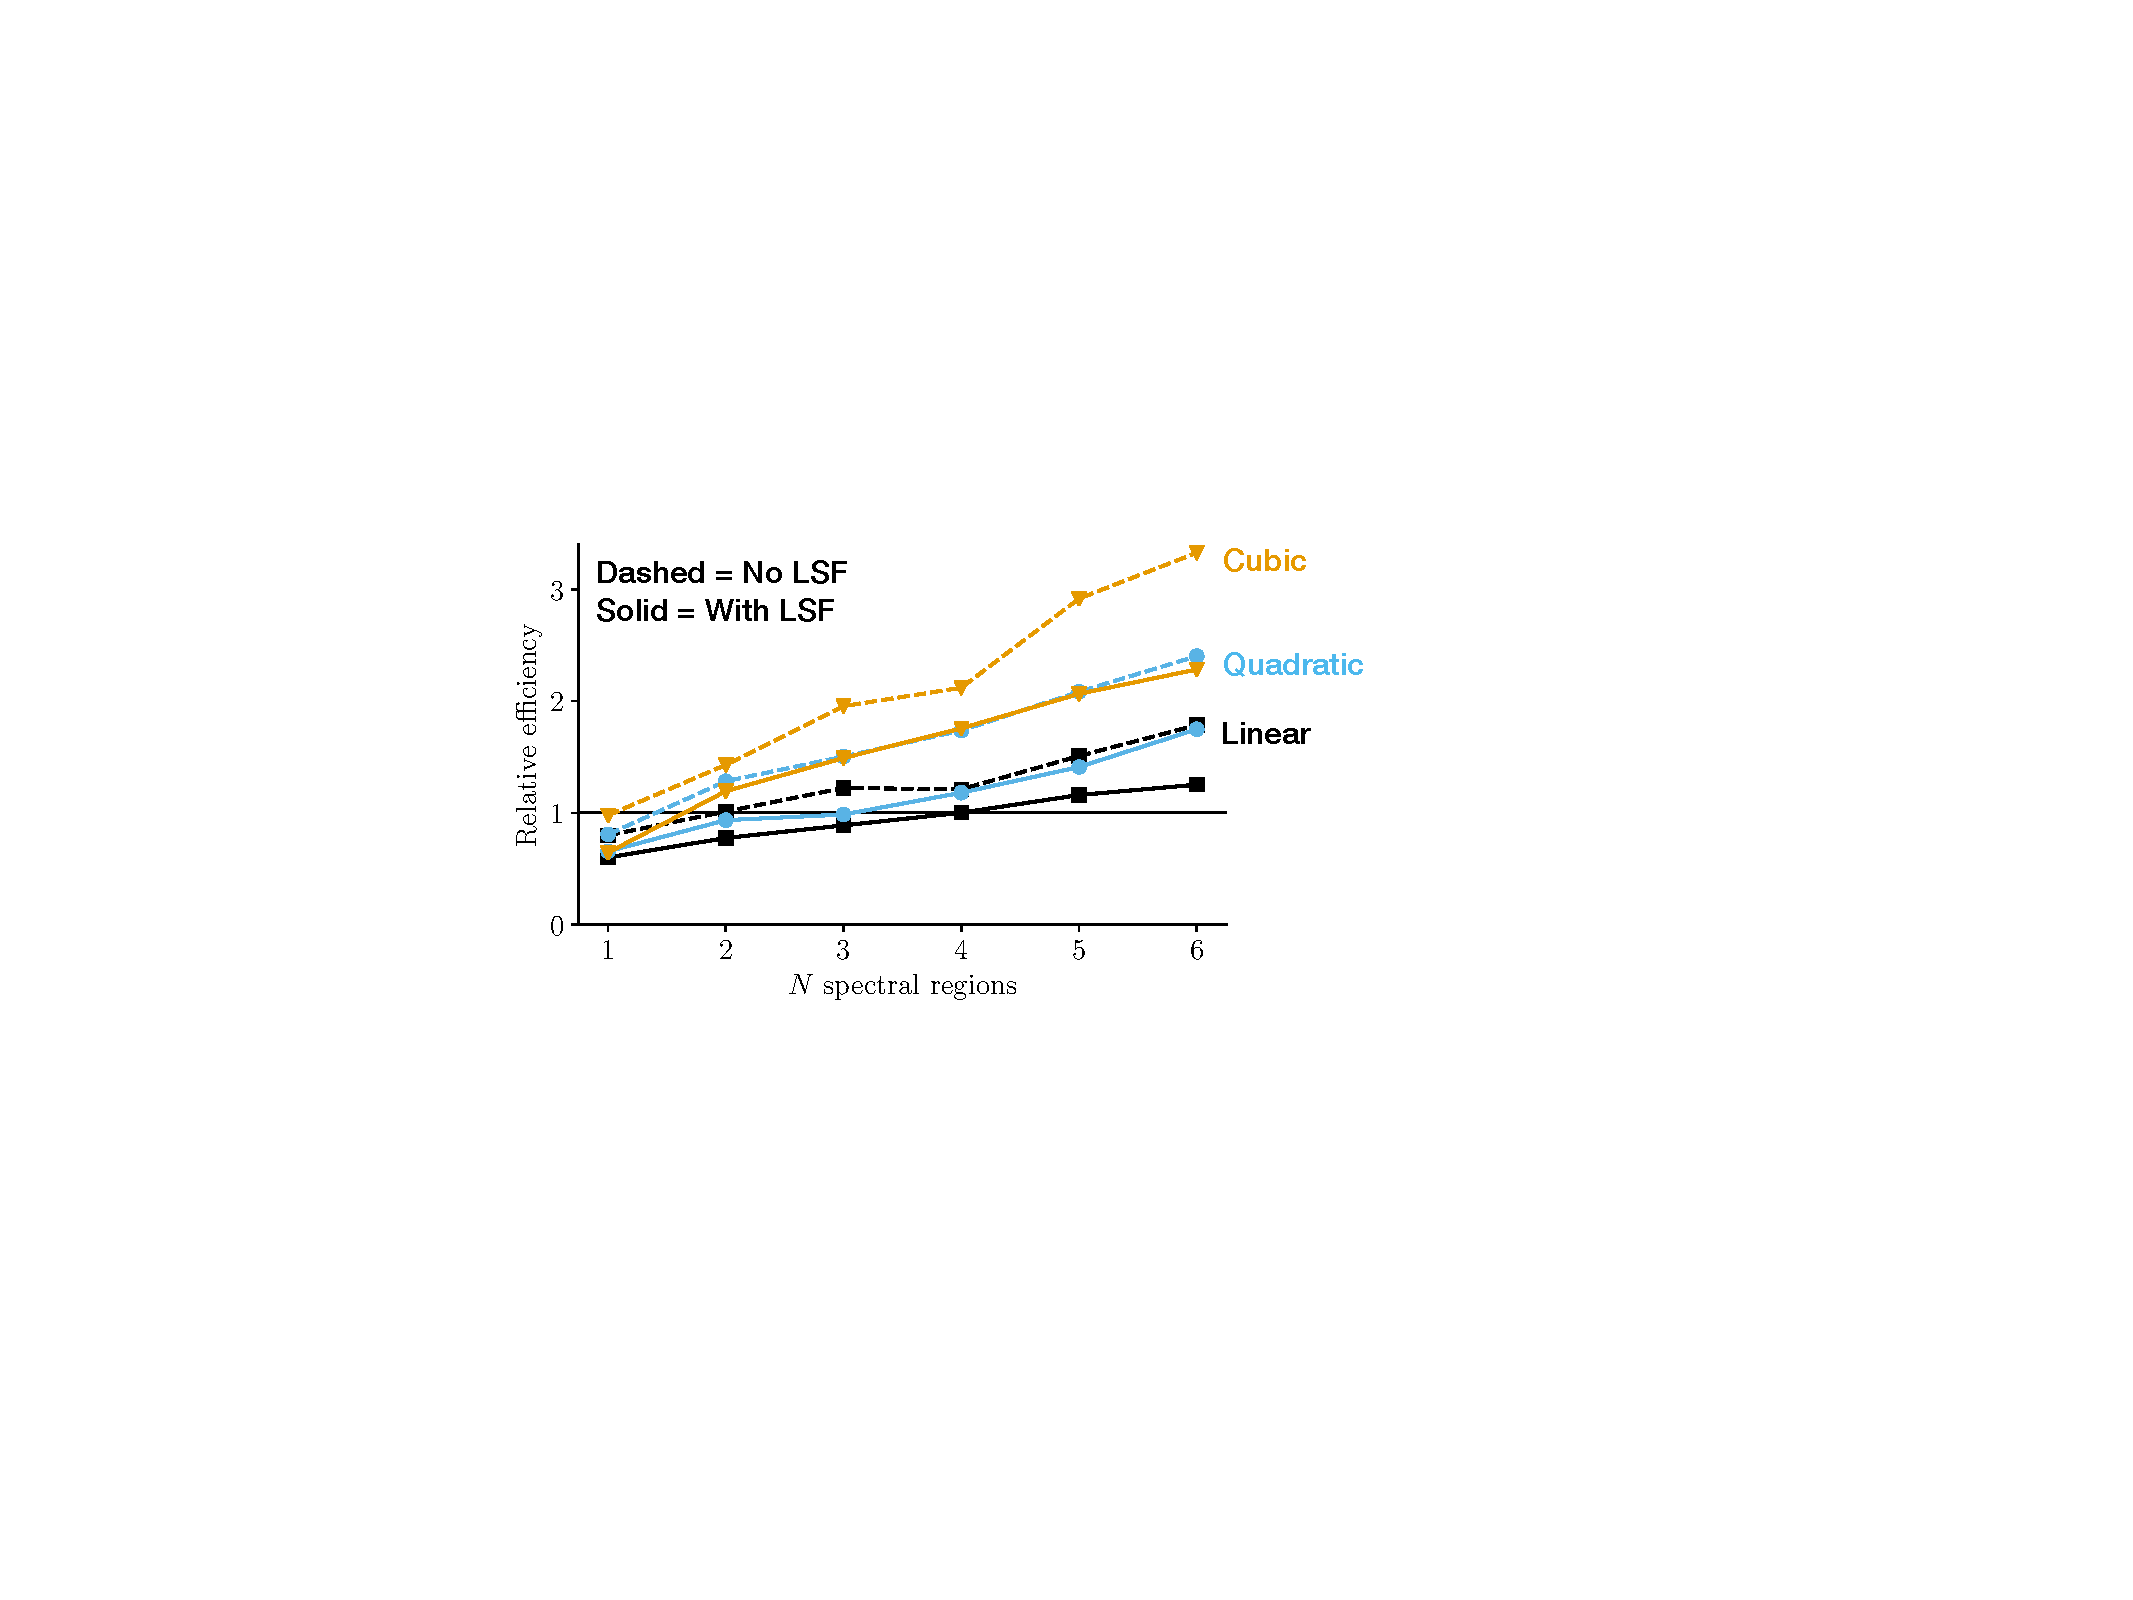
\includegraphics{efficiency.pdf}
  \caption{
  Relative efficiency of MCMC with analytic and numerical continuum parameter marginalization for absorption line analysis problems with different complexities.
  The relative efficiency is the ratio of the number of independent samples, $n_{\rm ind}$, generated in the same amount of time by the two marginalization approaches; $n_{\rm ind}^{(m)}$ uses the analytically marginalized likelihood, $n_{\rm ind}^{(u)}$ uses the unmarginalized likelihood.
  The larger the relative efficiency, the more independent samples generated by analytic marginalization.
  Line colors and markers correspond to different continuum parameterizations: degree 1 polynomial (black squares), degree 2 polynomial (blue circles), degree 3 polynomial (orange triangles).
  Line styles indicate whether a non-trivial LSF is used in the analysis.
  The relative efficiency is shown as a function of the number of spectral regions being analyzed simultaneously; each spectral region has its own set of continuum parameters.
  The relative efficiency and the problem setup are discussed in more detail in Section \ref{sec:MCMC-efficiency}.
  }
  \label{fig:efficiency-comparison}
\end{figure}

In ISM absorption spectra, it is common to have multiple lines in a spectrum with shared parameters.
These lines can be from the same species, e.g. the Lyman series, or from different species, e.g. from Mg {\tiny I}, Zn {\tiny II}, and Cr {\tiny II} which have overlapping lines in the near ultraviolet.
When these lines are in different parts of a spectrum, each part needs its own continuum parameters.
This is a case in which analytic marginalization can potentially be more efficient than MCMC marginalization.

We compare how quickly MCMC done using each of the two methods converges and how efficient MCMC done using each method is post-convergence.
Which comparison is more informative for choosing a method to use will depend on the purpose of the MCMC run.
If the goal of an MCMC run is to estimate some value at low-to-moderate precision, the rate of convergence will be the more important factor.
If the goal is instead to estimate some value at high precision, the burn-in period will usually be a small fraction of the total chain and post-convergency efficiency will be more important.

We consider a case where there are $N$ absorption lines with shared central velocities and widths and independent column densities.
Each absorption line is in a different spectral region.
The continuum in each spectral region is a polynomial of degree $M$.
The marginalized likelihood has $2 + N$ absorption line parameters.
The unmarginalized likelihood has $2 + N$ absorption line parameters and $N \times M$ continuum parameters.
We use the \texttt{emcee} implementation of the Goodman and Weare affine-invariant MCMC ensemble sampler to generate draws from the posterior corresponding to each of these likelihoods.
We use the minimum number of ``walkers,'' which is twice the number of parameters.

We use the Rubin-Gelman statistic $\hat{R}$ \citep{Gelman:1992zz} to assess convergence.
The Rubin-Gelman statistic compares the variance between and within different MCMC instances.
If the instances have all converged, these two variances should be approximately equal.
We run ten MCMC instances for 12800 (per-walker) steps and compute the Rubin-Gelman statistic from the second half of sub-chains of length $2^p \times 100$ for $p=0, 1, \ldots, 7$.
$\hat{R}$ is computed separately for each parameter.
Following common usage, we consider convergence to be reached when the $\hat{R}$ of all parameters is less than $1.1$.
We run this test for 1, 2, and 3 regions and absorption lines assuming a continuum of degree 1.
The value of the $\hat{R}$ as a function of (total) number of steps is shown in Figure \ref{fig:convergence-comparison}.
When there is a single region and line, the MCMC marginalization chain takes twice as many steps as the analytic marginalization chain to converge; when there are two regions, it takes eight times as many steps; when there are three, the MCMC marginalization chain has not converged by the maximum chain length of 12800 while the analytic marginalization chain converges within 1600 steps.

We use the number of independent samples per unit time to assess efficiency.
We run MCMC with the marginalized likelihood for 2000 burn-in steps and 8000 converged steps and record the average time per sample, $t_s$.
Because MCMC with the unmarginalized likelihood takes many steps to converge, we use draws from the converged part of the marginalized likelihood chain as a starting point; these draws only have values for the absorption line parameters.
At each set of absorption line parameters, we sample a set of continuum parameters from the conditional distribution discussed in Section \ref{sec:conditionals}.
From this starting point, we run MCMC with the unmarginalized likelihood for 4000 burn-in steps and 36000 converged steps and record the average time per sample.
We then compute the average integrated autocorrelation times $\tau_f$ of the walkers in both chains.
The number of independent samples per unit time is $n_i = \left(\tau_f \, t_s \right)^{-1}$.

We compute $n_i$ for a number of regions $N = 1, 2, \ldots, 6$, continua of polynomial degree $M=$ 1, 2, and 3, and either a trivial LSF or a banded LSF.
The ratio $n_{ind}^{(\text{m})} / n_{ind}^{(\text{u})}$ for each of these cases is shown in Figure \ref{fig:efficiency-comparison}.
When this ratio is greater than 1, running MCMC with the marginalized likelihood for a fixed amount of time will produce more independent samples than running MCMC with the unmarginalized likelihood for the same amount of time.
The greater the number of regions and the degree of the continuum, the greater the efficiency advantage of the marginalized likelihood over the unmarginalized likelihood.
This advantage will not depend on the number of datapoints in each spectral region so long as the LSF is trivial or banded, since in these cases the evaluation time of both likelihoods grows linearly with dataset length (see Section \ref{sec:scaling}).
}

\section{Implementation and demonstration}
\label{sec:package-and-demos}
In this Appendix, we describe how \pkgname{} is implemented (Section \ref{sec:implementation}), list some of its capabilities (Section \ref{sec:package-functionality}), and show how the computation time of different calculations grows with dataset and continuum model size (Section \ref{sec:scaling}).

\subsection{Implementation}
\label{sec:implementation}
We have implemented \pkgname{} as a pure-Python package with \texttt{numpy} and \texttt{scipy} as dependencies.
\pkgname{} does not contain functionality for building LSFs or computing transmittances from absorption parameters and is not intended to be a stand-alone analysis tool.
It is meant to be used as a drop-in likelihood function replacement in analysis packages or scripts.

\subsection{Package functionality}
\label{sec:package-functionality}
This package was designed for a use case where the log marginal likelihood and its gradient are evaluated at many different values of the $\theta$-dependent parameters (see Section \ref{sec:assumptions-and-formalism}) while the $\theta$-independent parameters are held constant.
The core feature of the package is the \texttt{MarginalizedLikelihood} class.
A \texttt{MarginalizedLikelihood} instance stores $\theta$-independent parts of the model and pre-computes quantities that are re-used during repeated marginalized likelihood evaluations.
In particular, it stores the data covariance matrix $\vx{K}$; the $\vx{c}$ prior covariance matrix $\vx{\Lambda}$ and its explicit inverse, if applicable; and the LSF mapping $\vx{L}$ and its transpose.

Both covariance matrices can be diagonal or fully general.
The package includes the \texttt{CovarianceMatrix} class, which defines a consistent interface for calculations, and two subclasses, \texttt{DiagonalCovarianceMatrix} and \texttt{GeneralCovarianceMatrix}.
\texttt{DiagonalCovarianceMatrix} wraps the simple, one-dimensional determinant and inverse calculations possible with a covariance matrix consisting purely of variances and does the book-keeping required to produce output with the correct shape.
\texttt{GeneralCovarianceMatrix} uses the Cholesky decomposition of the supplied covariance matrix to calculate its determinant and to left multipy matrices and vectors by its inverse.
Computing the Cholesky decomposition of a general covariance matrix of size $M$ by $M$ takes $\mathcal{O}(M^3)$ calculations, making it prohibitively computationally expensive for large $M$.

The LSF mapping $\vx{L}$ can be any object that implements the matrix multiplication interface, i.e. has a \texttt{matmul} or \texttt{\_\_matmul\_\_} method.
For example, $\vx{L}$ can be a dense matrix represented by a \texttt{numpy} array, a sparse matrix represented by a \texttt{scipy.sparse} matrix, or a convolution operator represented by a \texttt{scipy.sparse.linalg} \texttt{LinearOperator}.
$\vx{L}$ can also be the identity mapping (indicated by \texttt{None}), in which case it is left out of any likelihood calculations.


\subsection{Computation time as a function of dataset and basis size}
\label{sec:scaling}
The most time-consuming step in computing all of the quantities derived in Section \ref{sec:assumptions-and-formalism} is forming the matrix $\vx{C}_{n/u}$.
This step requires matrix-matrix products, while most other steps only involve matrix-vector products.
These expensive products are $\vx{L}\vx{B}$ and $\vx{K}^{-1} \left(\vx{L} \vx{B}\right)$.
The amount of time required to compute these products depends on the structure $\vx{L}$ and $\vx{K}$.

$\vx{L}$ can be the identity matrix, a dense matrix, a sparse matrix, or a linear mapping such as convolution.
The fastest case is when $\vx{L}$ is the identity matrix, since then $\vx{L}\vx{B}$ does not need to be computed.
The slowest case is when it is a dense matrix, in which case computation time grows as $\mathcal{O}(MN(P+Q))$.
When $\vx{L}$ is a sparse matrix or linear mapping, the scaling depends on its exact structure.
An LSF that varies with wavelength can be represented by a banded matrix, which will be sparse if the spectrum spans many resolution elements.
If the bandwidth of $\vx{L}$ is independent of the size of the dataset, the computation time of this product grows as $\mathcal{O}(M(P+Q))$.

We consider covariance matrices $\vx{K}$ that are either diagonal or general.
If $\vx{K}$ is diagonal, $\vx{K}^{-1} \left(\vx{L} \vx{B}\right)$ requires exactly $M(P+Q)$ multiplications.
When $\vx{K}$ is a general covariance matrix, we decompose it into its Cholesky factors and left-multiply $\vx{L} \vx{B}$ by $\vx{K}^{-1}$ by solving the linear problem $\vx{\vx{L} \vx{B}} = \vx{K} \vx{X}$.
The time needed to factor $\vx{K}$ grows as $\mathcal{O}\left(M^3\right)$ but only needs to be done once per set of observations.
The time needed to solve the linear problem grows as $\mathcal{O}\left(M^2 (P+Q)\right)$.

To empirically confirm these growth rates, we timed how long it takes to evaluate the log-likelihood and its gradient for a range of dataset sizes $M$ and basis sizes $P+Q$ and three $\vx{L}$ and $\vx{K}$ structure scenarios.
The scenarios are: $\vx{L}$ is the identity mapping, $\vx{K}$ is diagonal; $\vx{L}$ is a dense matrix, $\vx{K}$ is general; and $\vx{L}$ is a sparse, banded matrix and $\vx{K}$ is diagonal.
The first two scenarios are the fastest and slowest combination.
The third scenario is more typical for a spectrum; the data uncertainty is diagonal and the LSF has finite extent.
The evaluation time of the log-likelihood as a function of $M$ and $P+Q$ for these three scenarios is shown in Figures \ref{fig:uncorr-no-L-logp}, \ref{fig:corr-yes-L-logp}, and \ref{fig:uncorr-sparse-L-logp}.
We do not show the evaluation time of the gradient because it behaves in the same way as the evaluation time of the log-likelihood in all three scenarios; the most expensive step of the two calculations is the same.

The dependence of computation time on $M$ and $P+Q$ generally agrees with the predictions based on the two most time-consuming steps.
At low $M$ and in particular at low $P+Q$, the computation time is either overhead-dominated or evenly split between the most time-consuming steps and other steps.
When $M \gtrsim 10^5$, computation time increases faster than expected purely from the growth rate of the required number of operations (see e.g. the left panel of Figure \ref{fig:uncorr-no-L-logp}).
This excess increase in computation time is most likely due to changes in memory bandwidth, as the size of matrix rows and columns increases past the size of the highest-level CPU cache on the laptop used to run these tests.

To put these dataset sizes into context, a Sloan Digital Sky Survey (SDSS) BOSS or APOGEE spectrum is $\sim 10^3$ pixels long, a Hubble Space Telescope Cosmic Origins Spectrograph (HST-COS) spectrum is $\sim 10^4$ pixels long, and a spectrum from an echelle spectrograph such as the Ultraviolet and Visual Echelle Spectrograph on the Very Large Telescope or the Magellan Inamori Kyocera Echelle spectrograph is $\sim 10^5 - 10^6$ pixels long.
The uncertainties associated with these spectra are usually assumed to be diagonal and the LSFs are acceptably described by sparse, banded matrices, so the computation times given in Figure \ref{fig:uncorr-no-L-logp} and \ref{fig:uncorr-sparse-L-logp} should apply.

\begin{figure}
  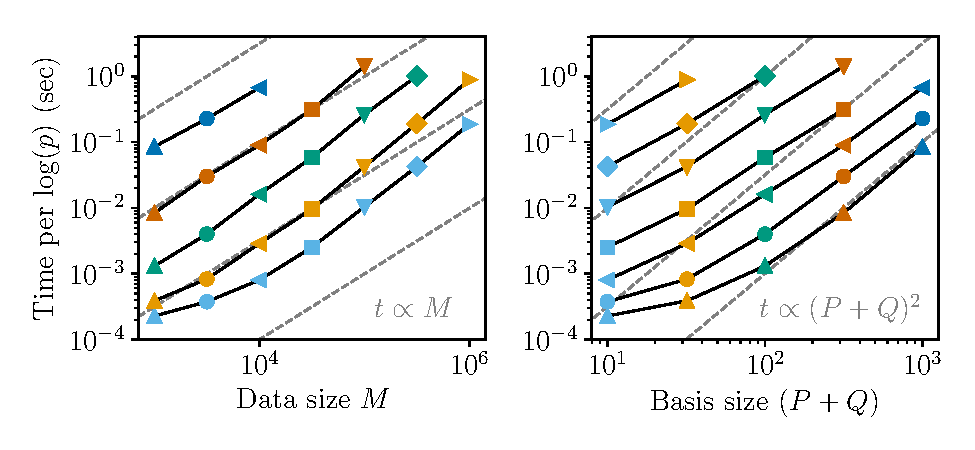
\includegraphics{uncorr_no_L_scaling.pdf}
  \caption{Computation time of the marginal log-likelihood (Equations \ref{eqn:proper-prior-marginal} and \ref{eqn:improper-prior-marginal}) when the data covariance matrix $\vx{K}$ is diagonal and $\vx{L}$ is the identity mapping as a function of dataset size $M$ (left panel) and basis size $P+Q$ (right panel). Values with the same marker shape were computed at the same dataset size $M$. Values with the same marker color were computed at the same dataset size $P+Q$. Polynomials of the form given in the bottom right corner of each panel are shown as dashed gray lines.}
  \label{fig:uncorr-no-L-logp}
\end{figure}

\begin{figure}
  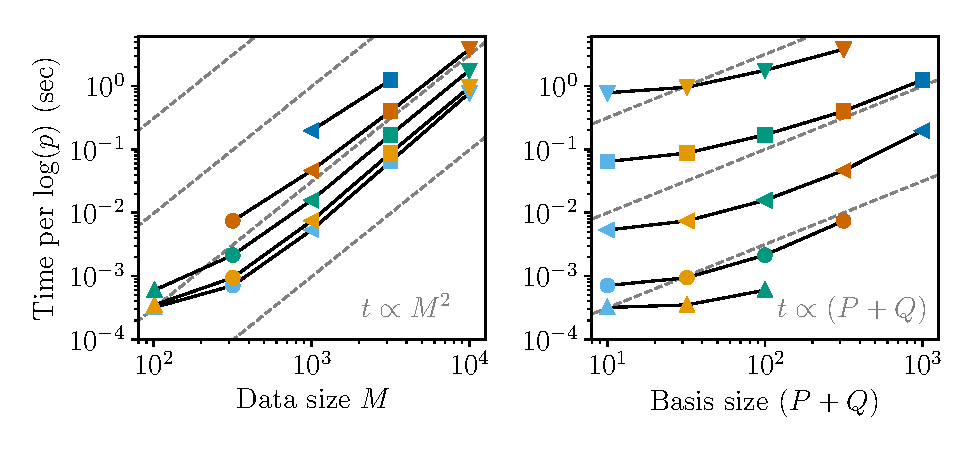
\includegraphics{corr_yes_L_scaling.pdf}
  \caption{Computation time of the marginal log-likelihood when the data covariance matrix $\vx{K}$ is not diagonal and $\vx{L}$ is a dense matrix. See caption of Figure \ref{fig:uncorr-no-L-logp} for a description of figure elements.}
  \label{fig:corr-yes-L-logp}
\end{figure}

\begin{figure}
  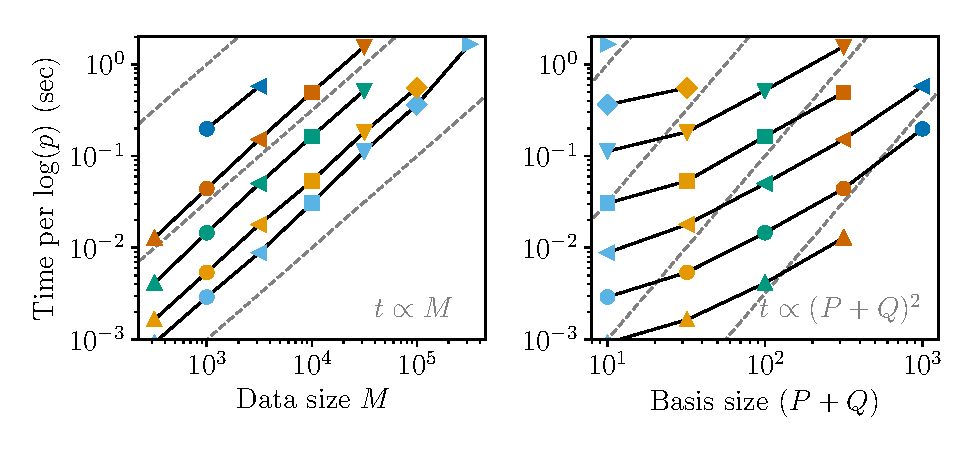
\includegraphics{uncorr_sparse_L_scaling.pdf}
  \caption{Computation time of the marginal log-likelihood when the data covariance matrix $\vx{K}$ is diagonal and $\vx{L}$ is a sparse, banded matrix. See caption of Figure \ref{fig:uncorr-no-L-logp} for a description of figure elements.}
  \label{fig:uncorr-sparse-L-logp}
\end{figure}

\bibliography{bibliography.bib}
%\bibliography{main.bbl}

\end{document}
